\documentclass{book}
\usepackage[ngerman]{babel}
\usepackage[utf8]{inputenc}
\usepackage{fancyhdr}
\usepackage{amsmath}
\usepackage{amsthm}
\usepackage{amssymb}
\usepackage{amsfonts}
\usepackage{mathtools}
\usepackage{xhfill}
\usepackage{xcolor}
\usepackage{graphicx}
\usepackage{float}
\usepackage{esint}
\usepackage{hyperref}
\usepackage[most]{tcolorbox}
\usepackage[chapter]{algorithm}
\usepackage{algpseudocode}


\graphicspath{ {./imgs/} }
\usepackage[
  a4paper,
  textwidth=175mm,
  textheight=225mm,
  heightrounded,
]{geometry}

\pagestyle{fancy}
\lhead{}
\chead{\thechapter. \chaptername}
\rhead{}
\lfoot{}
\cfoot{\thepage}
\rfoot{}

\author{Manuel Hinz}

\title{Einführung in die Grundlagen der Numerik (WS 22/23)}

\newtheorem{theorem}[algorithm]{Satz}
\newtheorem{corollary}[algorithm]{Korollar}
\newtheorem{lemma}[algorithm]{Lemma}
\newtheorem{definition}[algorithm]{Definition}
\newtheorem{remark}[algorithm]{Bemerkung}
\newtheorem*{mremark}{Eingefügte Bemerkung}
\newtheorem{example}[algorithm]{Beispiel}
\newtheorem*{mdefinition}{Eingefügte Definition}
\newtheorem*{mexample}{Eingefügtes Beispiel}



\def\C{\mathbb{C}}
\def\R{\mathbb{R}}
\def\N{\mathbb{N}}
\def\Z{\mathbb{Z}}
\def\rang{\text{rang}}
\def\cond{\text{cond}}
\def\eps{\text{eps}}
\raggedright

\let\cleardoublepage=\clearpage

\begin{document}

    \maketitle

    \tableofcontents

    \section*{Vorwort}

            Diese Mitschrift von der Vorlesung Einführung in die Grundlagen der Numerik (Dölz,WS 2022/2023) 
            wird von mir neben der Vorlesung geschrieben und ist dementsprechend Fehleranfällig. Fehler gerne an 
            mh@mssh.dev! 

    \chapter{Orthogonalität}

        \section{Grundlegende Definitionen}

            \begin{definition}\label{d1.1}
                Sei $X$ ein $\R$ Vektorraum und $\langle\cdot,\cdot\rangle:X\times X \to \R$ eine Abbildung. $\langle\cdot,\cdot\rangle$ heißt \textbf{Skalarprodukt} oder inneres Produkt, falls
                \begin{equation}
                    \tag{Positiviät}
                    \forall f\in X\setminus 0: \langle f,f \rangle>0
                \end{equation}
                \begin{equation}
                    \tag{Symmetrie}
                    \forall f,g\in X: \langle f,g \rangle = \langle g,f \rangle
                \end{equation}
                \begin{equation}
                    \tag{Linearität im ersten Argument}
                    \forall \alpha,\beta\in\R, f,g,h\in X: \langle \alpha f+\beta g,h \rangle
                    = \alpha \langle f,h \rangle + \beta \langle g,h \rangle
                \end{equation}
            \end{definition}

            \begin{remark}\label{b1.2}
                Symmetrie und Linearität im ersten Argument implizieren, 
                dass $\langle \cdot,\cdot  \rangle$ eine bilineare Abbildung ist. 
            \end{remark}

            \begin{definition}\label{d1.3}
                Sei $X$ ein $\R$-Vektorraum mit Skalarprodukt $\langle \cdot,\cdot \rangle$.
                Wir bezeichnen die zugehörige \textbf{Norm} (in Abhänigkeit von einem Vektor $f\in X$) mit 
                \begin{equation*}
                    \Vert f \Vert =\sqrt{\langle f,f\rangle}.
                \end{equation*}
            \end{definition}

            \begin{lemma}\label{l1.4}
                Sei $X$ ein $\R$-Vektorraum mit Skalarprodukt $\langle \cdot,\cdot \rangle$. Dann gil die \underline{Cauchy-Schwarz-Ungleichung}:
                \begin{equation}
                    \tag{C.S.}
                    \forall f,g\in X:\langle f,g \rangle\leq \Vert f\Vert \cdot\Vert g \Vert
                \end{equation}
                mit Gleichheit genau dann, wenn $f$ und $g$ linear abhängig sind.
            \end{lemma}
            \begin{proof}
                O.B.d.A. $f,g\neq 0$, da sonst offensichtlich Gleichheit gilt.
                Sei $\alpha\neq 0$, dann gilt mit $f,g\in X$ und $\alpha \in \R$:
                \begin{equation*}
                    0\leq \Vert f -\alpha g\Vert^2= \langle f-\alpha g,f-\alpha g \rangle
                    = \Vert f \Vert^2 -2\alpha \langle f,g \rangle+\alpha^2 \Vert g \Vert^2
                \end{equation*}
                Wählen wir jetzt $\alpha=\frac{\langle f,g \rangle}{\Vert g \Vert^2}$ folgt:
                \begin{equation*}
                    0\leq \Vert f \Vert^2-\frac{2 \langle f,g \rangle^2}{\Vert g \Vert^2}+\frac{\langle f,g \rangle^2}{\Vert g \Vert^2}
                \end{equation*}
                \begin{equation*}
                    \implies \langle f,g \rangle^2\leq \Vert f \Vert^2\cdot \Vert g \Vert^2.
                \end{equation*}
            \end{proof}
            \begin{mremark}
                Rechnung zur Begründung von $ \langle f-\alpha g,f-\alpha g \rangle
                = \Vert f \Vert^2 -2 \Vert\alpha \langle f,g \rangle+\alpha^2 \Vert g \Vert^2$:
                \begin{align*}
                    &\langle f-\alpha g,f-\alpha g \rangle\\
                    &=\langle f,f-\alpha g \rangle-\alpha \langle g,f-\alpha g \rangle\\
                    &=\langle f,f \rangle-\alpha \langle f,g \rangle-\alpha \langle g,f \rangle+\alpha^2 \langle g,g \rangle\\
                    &=\Vert f \Vert^2 -2 \Vert\alpha \langle f,g \rangle+\alpha^2 \Vert g \Vert^2
                \end{align*}
            \end{mremark}
            \begin{example}\label{b1.5}
                \begin{enumerate}
                    \item $X=\R^n$ und $\langle x,y \rangle=\sum_{i=1}^n x_iy_i$ (Euklidisches Skalarprodukt)
                    \item $X=\R^n$, $\langle x,y \rangle=x^\perp A y$, wobei $A$ positiv definit und symmetrisch ist
                    \item $I=[a,b],w:I\to\R$ beschränkt und strikt positiv:
                        \begin{equation*}
                            X=\left\{f:I\to\R:\int_a^b f(x)^2w(t)dt<\infty\right\}=L^2(I,w)
                        \end{equation*}
                        mit 
                        \begin{equation*}
                            \langle f,g \rangle = \int_a^b f(t)g(t)w(t)dt
                        \end{equation*}
                \end{enumerate}
            \end{example}
            \begin{mremark}
                Die Definition von $L^2(I,w)$ ist hier nicht ganz richtig, man müsste natürlich noch Äquivalenzklassen, bzgl. Gleichheit bis auf Nullmengen, bilden. 
                Dies wird hier, da Analysis 3 / Wtheo. nicht nicht vorrausgesetzt wird, ignoriert.
            \end{mremark}
            \begin{definition}\label{d1.6}
                Sei $X$ ein $\R$-VR mit Skalarprodukt $\langle \cdot,\cdot \rangle$.
                $f,g\in X$ heißen \textbf{orthogonal}, falls $\langle f,g \rangle=0$.
            \end{definition}
            \begin{remark}\label{b1.7}
                Im $\R^n$ mit dem euklidischen Skalarprodukt stimmt Definition \ref*{d1.6}, wegen 
                \begin{equation*}
                    \langle x,y \rangle = \Vert x \Vert \Vert y \Vert \cos(\theta), \theta=\angle(x,y),
                \end{equation*}
                mit unserem bisherigen Verständnis überein.
            \end{remark}
        \section{Bestapproximationseigenschaft}
            \begin{definition}\label{d1.8}
                Sei $V$ ein $\R$-VR mit Skalarprodukt $\langle \cdot,\cdot \rangle$ und $U$ ein Unterraum.
                \begin{equation*}
                    U^\perp = \left \{ v\in V: \langle v,u \rangle=0,\forall u\in U\right\}
                \end{equation*}
                heißt das \textbf{orthogonale Komplement} von $U$.
            \end{definition}
            \begin{theorem}\label{s1.9}
                Unter den Annahmen von Definition \ref*{d1.8} und der  zusätzlichen Annahme, dass $U$ endlich dimensional ist, gilt folgendes für $v\in V$:
                \begin{equation*}
                    \Vert v-u \Vert = \min_{w\in U}\Vert v-w\Vert
                \end{equation*}
                genau dann, wenn $v-u\in U^\perp$.
            \end{theorem}
            \begin{example}\label{b1.10}
                $V=\R^2$, $U=\text{span}\left\{\begin{pmatrix}1\\1\end{pmatrix}\right\}$ mit euklidischem Skalarprodukt $\langle \cdot,\cdot \rangle$.
                Dann ist $U^\perp = \text{span}\left\{\begin{pmatrix}1\\-1\end{pmatrix}\right\}$. 
                \begin{figure}[H]
                    \centering
                    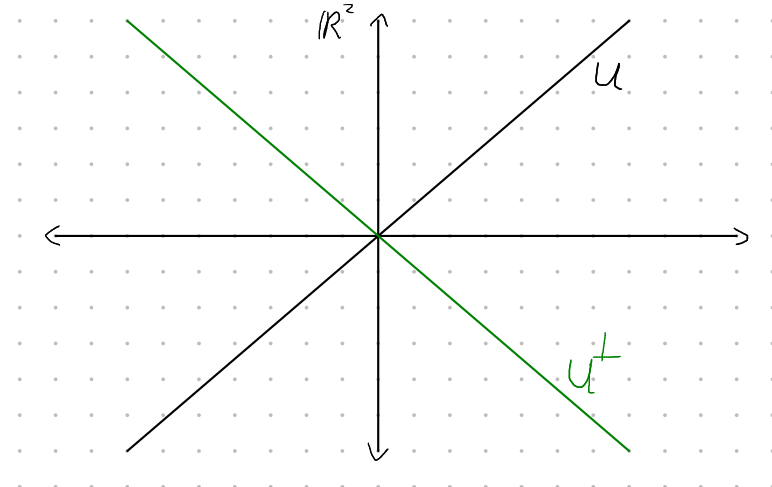
\includegraphics[width=0.25\textwidth]{Bild001}
                    \caption{\(U\) und \(U^\perp\)}
                \end{figure}
            \end{example}
            \begin{proof}[Beweis von Satz \ref*{s1.9}]
                Sei $v\in V$ und seien $u,w\in U$. Dann gilt:
                \begin{equation*}
                    \Vert v-w \Vert^2=\langle v-w,v-w \rangle = \langle (v-u)+(u-w),(v-u)+(u-w) \rangle
                \end{equation*}
                \begin{equation*}
                    =\Vert v-u \Vert^2+2 \langle v-u,\underbrace{u-w}_{\in U} \rangle +\Vert u-w \Vert^2\geq \Vert v-u \Vert^2
                \end{equation*}
                mit Gleichheit genau dann, wenn $w-u=0$ (da dann der $\Vert u-w \Vert$ Term verschwindet).
            \end{proof}
            \begin{remark}\label{b1.11} 
                Der Satz sagt, dass es zu \underline{jedem} $v\in V$ ein \underline{eindeutiges, bestmögliches} $u\in U$ gibt.
            \end{remark}
            \begin{definition}\label{d1.12} 
                Die Lösung aus Satz \ref*{s1.9} heißt \textbf{orthogonale Projektion} von $v$ auf $U$. Die Abbildung 
                \begin{equation*}
                    P:V\to U, v\mapsto P(v) \textbf{ mit } \Vert v-Pv \Vert=\min_{w\in U}\Vert v-w \Vert
                \end{equation*}
                ist linear und wird \textbf{orthogonale Projektion} genannt.
            \end{definition}
            \begin{mremark}[Beweis der Linearität]
                Für $v_1,v_2\in V$ und $\alpha\in \R$ gilt:
                \begin{align*}
                    v_1-Pv_1\in U^\perp\\
                    v_2-Pv_2\in U^\perp 
                \end{align*}
                Daher 
                \begin{align*}
                    \alpha(v_1-Pv_1)+(v_2-Pv_2)=(\alpha v_1+v_2) - (\alpha Pv_1 + Pv_2) \in U^\perp.
                \end{align*}
                Aber dann muss $\alpha Pv_1+Pv_2$ schon, wegen der Eindeutigkeit, $P(\alpha v_1+v_2)$ sein.
            \end{mremark}
            \begin{remark}\label{b1.13}
                Satz \ref{s1.9} gilt auch, wenn $U$ durch $W=w_0+U$ ersetzt wird.
                Die orthogonale Projektion ist analog definiert..
            \end{remark}

            \underline{\textbf{Frage:}} Die Orthogonale Projektion hat offenbar gute Eigenschaften. Aber: wie berechnen wir sie? Wie wählen wir $U$?
            
            \begin{itemize}
                \item Berechnung ist leicht
                \item U wählen schwierig
            \end{itemize}

        \section{Orthonormalbasen}

            \begin{definition}\label{d1.14}
                Sei $X$ ein $\R$-VR mit Skalarprodukt $\langle \cdot,\cdot \rangle$ und
                $X_n\subset X$ ein endlich dimensionaler Teilraum mit Basis $\{\varphi_1,\dots,\varphi_n\}$.
                Die Basis heißt \textbf{Orthogonalbasis}, falls 
                \begin{equation*}
                    \forall i\neq j: \langle \varphi_i,\varphi_j \rangle=0
                \end{equation*}
                gilt und Orthonormalbasis (ONB), falls zusätzlich $\Vert\varphi_i\Vert=1$ gilt. Das impliziert:
                \begin{equation*}
                    \langle \varphi_i,\varphi_j \rangle =\delta_{i,j}.
                \end{equation*}
            \end{definition}

            \begin{example}\label{b1.15}    
                \begin{enumerate}
                    \item $\R^n$ mit euklidischem Skalarprodukt und kanonischer Basis
                    \item $X=L^2(I,1)$ mit entsprechendem Skalarprodukt und $X_n$ der Raum der trigonometrischen Polynome bis Grad $n$.
                    Dann ist folgendes eine ONB:
                    \begin{equation*}
                        \left\{\frac{1}{\sqrt{2\pi}},\frac{\sin(x)}{\sqrt{\pi}},\frac{\cos(x)}{\sqrt{\pi}},\dots,\frac{\sin(nx)}{\sqrt{\pi}},\frac{\cos(nx)}{\sqrt{\pi}}\right\}
                    \end{equation*}
                \end{enumerate}
            \end{example}

            \begin{mremark}
                Trigonometrische Polynome sind Funktionen der Form
                \begin{equation*}
                    f(t)=\sum_{k=1}^n a_k \cos(kx)+ b_k \sin(kx).
                \end{equation*}
                Die größte Faktor vor dem $x$ ist der Grad eine trigonometrischen Polynoms.
            \end{mremark}

            \begin{theorem}\label{s1.16}
                Sei $\{\varphi_1,\dots,\varphi_n\}$ eine ONB von $X_n\subset X$. Dann gilt
                \begin{enumerate}
                    \item $f=\sum_{i=1}^n \langle \varphi_i,f \rangle\varphi_i$
                    \item $\Vert f \Vert^2=\sum_{i=1}^n \langle \varphi_i,f \rangle^2$
                    \item Die orthogonale Projektion $f_n$ von $f\in X\setminus X_n$ ist gegeben durch 
                        \begin{equation*}
                            f_n=\sum_{i=1}^n \langle \varphi_i,f \rangle\varphi_i
                        \end{equation*}
                    \item im Fall von 3.:
                        \begin{equation*}
                            \Vert f_n \Vert^2 = \sum_{i=1}^n \langle \varphi_i,f \rangle^2 \leq \Vert f \Vert
                        \end{equation*}
                \end{enumerate}
            \end{theorem}
            
            \begin{proof}
                1.: 
                \begin{align*}
                    &f\in X_n\implies \exists \alpha_i\in \R: f=\sum_{i=1}^n\alpha_i\varphi_i\\
                    &\implies \langle \varphi_i,f \rangle= \langle \varphi_i, \sum_{j=1}^n\alpha_j\varphi_j\rangle
                    =\sum_{j=1}^n \alpha_j \langle \varphi_i,\varphi_j \rangle =\alpha_i
                \end{align*}
                2.:
                \begin{align*}
                    &\Vert f \Vert^2 = \langle f,f \rangle \\
                    &= \langle \sum_{i=1}^n \alpha_i \varphi_i, \sum_{j=1}^n \alpha_j \varphi_j \rangle =\sum_{i,j=1}^n\alpha_i\alpha_j\delta_{i,j}=\sum_{i=1}^n\alpha_i^2
                \end{align*}
                3.:
                \begin{align}
                    f\in X\setminus X_n:&\nonumber\\
                    \Vert f-\underbrace{\tilde{f}_n}_{\in X_n} \Vert &= \langle f-\sum_{i=1}^n\tilde{\alpha}_i\varphi_i,f-\sum_{i=1}^n\tilde{\alpha}_i\varphi_i \rangle\nonumber\\
                    &=\Vert f \Vert^2-2\sum_{i=1}^n\tilde{\alpha}_i \underbrace{\langle \varphi_i,f \rangle}_{\eqqcolon \alpha_i}+\sum_{i,j=1}^n\alpha_i\alpha_j \langle \varphi_i,\varphi_j \rangle \nonumber\\
                    &=\Vert f \Vert^2-\sum_{i=1}^n\tilde{\alpha}_i\alpha_i+\sum_{i=1}^n\tilde{\alpha}_i^2
                    \stackrel{\text{Quadratische Ergänzung}}{=} \Vert f \Vert^2-\sum_{i=1}^n\alpha_i^2+\sum_{i=1}^n\underbrace{(\alpha_i-\tilde{\alpha}_i)^2}_{\geq 0}
                \end{align}
                Dies wird minimiert, wenn $\tilde{\alpha}_i=\alpha_i$ ist.
                
                4.:

                $f\in X_n$ wurde in 2. gezeigt. Sonst:
                \begin{equation*}
                    f\notin x_n\implies \text{ mit } \alpha_i=\tilde{\alpha}_i \text{ in } (1.1):
                \end{equation*}
                \begin{equation*}
                    0\leq \Vert f-f_n \Vert^2=\Vert f \Vert^2-\sum_{i=1}^n\underbrace{\alpha_i^2}_{\langle \varphi_i,f \rangle^2}
                \end{equation*}
                Es folgt die Behauptung.
            \end{proof}

            \underline{\textbf{Vorteile von Orthogonalität:}}
            \begin{itemize}
                \item Bestapproximation
                \item Einfache Basisdarstellung
            \end{itemize}

        \noindent
        \xrfill[0.7ex]{1pt}Ende von Vorlesung 01 am 11.10.2022\xrfill[0.7ex]{1pt}

    \chapter{Das lineare Ausgleichsproblem}

        \section{Problemstellung und Normalengleichung}

            Gegeben seien Punkte $(t_i,b_i)\in\R^2$ mit $i=1,\dots,m$. Wir nehmen an, dass es eine Gestzmäßigkeit im Sinne eines
            parameterabhängigen Modelles 
            \[
                b_i=b(t_i)=b(t_i;\underbrace{x_1,\dots,x_n}_{\text{Parameter}}),
            \]
            wobei die Parameter $x_1,\dots,x_n$ unbekannt seien, gibt. In der Praxis sind die Messungen zusätzlich mit Fehlern
            behaftet und das Modell gilt nur approximativ. Zusätzlich gibt es oft mehr Messungen als Parameter, d.h. $m>n$.

            \underline{\textbf{Frage:}} Gegeben die Messungen, können wir zugehörige Parameter bestimmen?

            \underline{\textbf{Annahme:}} $b$ ist linear in den Parametern, d.h. es gibt Funktionen 
            \[a_i:\R\to\R\]
            s.d.
            \[b(t;x_1,\dots,x_n)=a_1(t)x_1+\dots+a_n(t)x_n.\]
            \underline{\textbf{Idee:}} Formuliere ein lineares Gleichungssystem:
            \[b_i \approx b(t_i;x_1,\dots,x_n)=a_1(t_i)x_1+\dots+a_n(t_i)x_n, i=1,\dots,m\]
            kurz $Ax\approx b$ mit $A\in\R^{m\times n},x\in\R^n,b\in\R^m$.

            \underline{\textbf{Problem:}} Durch Modell- und Messfehler gilt das Gleichungssystem nur ungefähr, und wir 
            mehr Gleichungen als Unbekannte (``das Gleichungssystem ist überbestimmt''). Wir können unser Gleichungssystem 
            also im Allgemeinen nicht lösen.

            \begin{example}\label{b2.1}
                \begin{figure}[H]
                    \centering
                    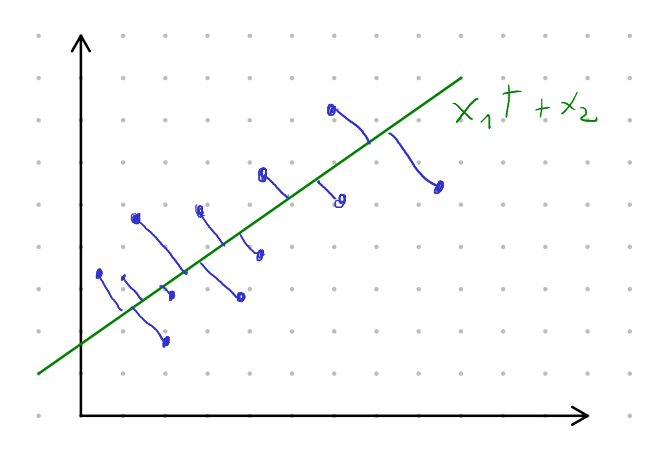
\includegraphics[width=0.25\textwidth]{Bild002}
                    \caption{Datenpunkte und approximierte Gerade}
                \end{figure}
            \end{example}

            \underline{\textbf{Idee:}} Finde Parameter, sodass das Modell ``bestmöglich'' mit den Messpunkten übereinstimmt, 
            d.h. finde $(x_1,\dots,x_n)^t=x\in\R^n$ s.d.:
            \begin{equation}\label{g2.1}
                \Vert Ax-b \Vert=\min_{y\in\R^n} \Vert Ay-b \Vert
            \end{equation}
            
            \begin{definition}\label{d2.2}
                Die Gleichung (\ref{g2.1}) heißt \textbf{lineares Ausgleichsproblem}. Der Term $Ax-b$ heißt \textbf{Residuum}.
            \end{definition}

            \underline{\textbf{Bemerke:}} $V=\R^m,U=\text{Bild}(A)\subset V,\dim(\text{Bild}(A))\underbrace{\leq n\leq m}_{\text{Grundannahme}}$

            Statte $V$ mit euklidischem Skalarprodukt aus.

            $\stackrel{Satz \ref{s1.9}}{\implies}$ Es gibt genau ein $Ax\in$ Bild$(A)$ so, dass
            \[\Vert Ax-b \Vert=\min_{w\in U} \Vert w-b \Vert\]
            gilt.

            \underline{\textbf{Aber:}} Wie berechnen wir $x$?

            \begin{theorem}\label{s2.3}
                Sei $A\in\R^{m\times n},b\in\R^m,m\geq n,x\in\R^n$ ist genau dann eine Lösung von (\ref{g2.1}) 
                bezüglich der euklidischen Norm, falls
                \begin{equation}\label{g2.2}
                    A^tAx=A^tb.
                \end{equation}
                Insbesondere ist das lineare Ausgleichproblem genau dann lösbar, falls $\rang(A)=n$.
            \end{theorem}

            \begin{proof}
                \begin{align*}
                    &\Vert Ax-b \Vert=\min_{y\in\R^n} \Vert Ay-b \Vert\\
                    &\stackrel{\text{Satz } (\ref{s1.9})}{\iff}Ax-b\in U^\perp=\text{Bild}(A)^\perp\\
                    &\iff \forall y\in\R^n: \langle Ax-b, Ay\rangle=0\\
                    &\iff \forall y\in\R^n: \langle A^tAx-A^tb,y \rangle=0\\
                    &\iff A^tAx=A^tb
                \end{align*}
                Die letzte Gleichung ist genau dann invertierbar, wenn $A^tA$ vollen Rang hat, also wenn $A$ vollen Rang ($n$) hat.
            \end{proof}

            \begin{remark}\label{b2.4}
                Im beweis verwenden wir, dass $Ax-b$ orthogonal zu $U=\text{Bild}(A)$,

                    \begin{figure}[H]
                        \centering
                        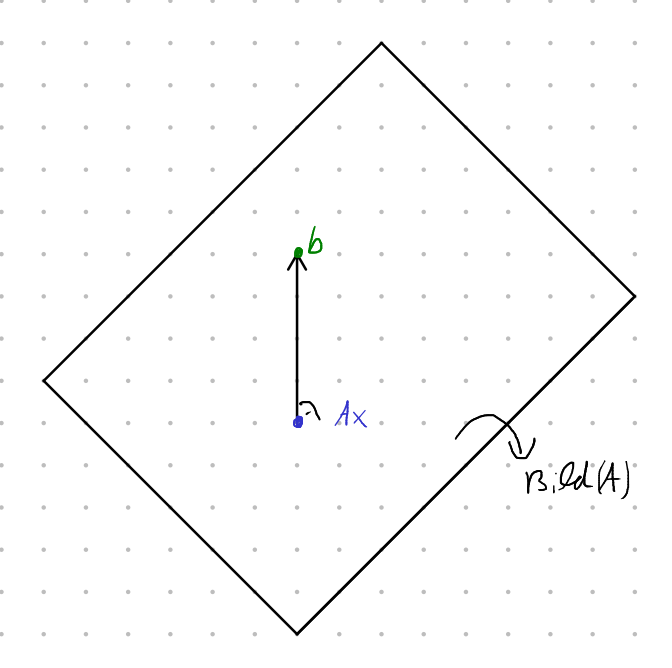
\includegraphics[width=0.25\textwidth]{Bild003}
                        \caption{Hyperebene und Projektion}
                    \end{figure}

                d.h. eine Normale zur Hyperebene Bild$(A)$ im $R^m$, ist. Deshalb heißt (\ref{g2.2}) auch \textbf{Normalengleichung}.
            \end{remark}

            \begin{remark}\label{b2.5}
                Für $m=n$ und $\rang(A)=n$ ist die Lösung des linearen Ausgleichproblems exakt (im mathematischen Sinne).
            \end{remark}

            \begin{theorem}\label{s2.6}
                Für $A\in\R^{m\times n}$ ist $A^tA$ symmetrisch und positiv semidefinit. Falls $m\geq n$ ist $A^tA$ genau 
                dann positiv definit, wenn $\rang(A)=n$.
            \end{theorem}
            \begin{proof}
                \begin{itemize}
                    \item Symmetrisch: klar
                    \item positiv semidefinit:
                    \[\forall x\in \R^n: x^t(A^tA)x=(Ax^t)(Ax)=\Vert Ax \Vert_2^2\geq 0\]
                    \item positiv definit: $\rang(A)=n\implies Ax=0\iff x=0\implies \Vert Ax \Vert_2=0\iff x=0\implies $ Behauptung.
                \end{itemize}
            \end{proof}
        
        Einfachste Möglichkeit zur Lösung von (\ref{g2.2}): Berechne $A^tA,A^tb$, löse LGS mittels Cholesky. Kosten sind ungefähr:
        \[\frac{n^2m}{2}+m\cdot n+\frac{n^3}{6}+\frac{n^2}{2}+\frac{n^2}{2}\approx\frac{mn^2}{2} \text{ für } m\gg n.\]
        
        \begin{mremark}
            Anmerkung vom Donzent: $A^tA$ eig. immer schlecht zu berechnen.
        \end{mremark}

        %Hier Konditionierung nacharbeiten

        \underline{\textbf{Aber:}} Dieser Vorgang ist schlechter konditioniert als das lineare Ausgleichsproblem: 
        
        \begin{tcolorbox}[enhanced,breakable,
            title=Eingeschobene Definition / Wiederholung]
            \[
                \cond(A)=\Vert A \Vert \Vert A^{-1} \Vert
            \]
            \[
                \Vert A \Vert =\max_{\Vert x \Vert=1} \Vert Ax \Vert
            \]
        \end{tcolorbox}

        Falls $A\in\R^{n\times n}$ spd (symmetrisch, positiv definit) gilt $\cond_2((A^tA))=\cond_2(A)^2$. 

        Für $A\in\R^{m\times n}$ gelten ähnliche Überlegungen, siehe Deuflhard \& Hohmann.

        \begin{example}\label{b2.7}
            Sei $A=\begin{bmatrix}
                1 & 1\\\epsilon&0\\0 & \epsilon
            \end{bmatrix}$ mit $\epsilon>\underbrace{\eps}_{\text{Maschienengenauigkeit}},\epsilon^2<\eps$.
            \[\implies A^tA=\begin{bmatrix}
                1 +\epsilon^2 & 1\\
                1 & 1+\epsilon^2
            \end{bmatrix}\stackrel{\text{im Computer}}{=}\begin{bmatrix}
                1 & 1\\
                1 & 1
            \end{bmatrix}\]
            $\implies$ $A^tA$ ist im Computer singulär, obwohl A vollen Rang hat!
        \end{example}

        \underline{\textbf{Idee / Wunsch:}} Gebe einen Algorithmus an, der das lineare Ausgleichsproblem löst und nur 
        auf $A$ arbeitet.

        \section{Methode der Orthogonalisierung}

            \begin{definition}\label{d2.8}
                Eine Matrix $Q\in\R^{n\times n}$ heißt \textbf{orthogonal}, wenn $Q^tQ=I$, d.h. falls die Spalten von $Q$ eine ONB bzgl. des 
                euklidischen Skalarprodukts bilden. Schreibe $Q\in O(n)$.
            \end{definition}

            \underline{\textbf{Notation:}} $\langle \cdot,\cdot \rangle_2,\Vert \cdot \Vert_2$ für das euklidische Skalarprodukt / die euklidische Norm.

            \begin{lemma}\label{l2.9}
                Für alle $Q\in O(n)$ gilt
                \begin{enumerate}
                    \item $\Vert Qx \Vert_2=\Vert x \Vert_2$ (Invarianz der Norm bzgl. orthogonaler Projektionen)
                    \item $\cond_2(Q)=1$
                \end{enumerate}
            \end{lemma}

            \begin{proof}
                1.: $\Vert Qx \Vert_2^2=\langle Qx,Qx \rangle_2=\langle Q^tQx,x \rangle_2=\langle x,x \rangle_2=\Vert x \Vert_2^2$

                2.: $\Vert Q \Vert_2=\max_{\Vert x \Vert_2=1}\Vert Qx \Vert=1$ und auch $\Vert Q^-1 \Vert_2=1\implies$ Behauptung.
            \end{proof}

            \begin{theorem}\label{s2.10}
                $A\in\R^{m\times n},m\geq n,\rang(A)=n$. Dann hat $A$ eine QR-Zerlegung:
                \begin{equation*}
                    A=Q\begin{pmatrix*}
                        R\\
                        0
                    \end{pmatrix*}
                \end{equation*}
                wobei $Q\in O(m),R\in\R^{n\times n}$ eine obere Dreiecksmatrix ist.
            \end{theorem}

            \begin{proof}
                Schreibe das Gram-Schmidt-Orthogonalisierungsverfahren in Matrixform:
                \[
                Q=\underbrace{\begin{bmatrix}
                    &&&\\
                    &&&\\
                    &&&\\
                    A_n & \dots & A_2 & A_1\\
                    &&&\\
                    &&&\\
                    &&&
                \end{bmatrix}
                \underbrace{
                \begin{bmatrix}
                    1 & \dots  & \dots & \dots & \frac{-\langle A_n,A_1 \rangle_2}{\Vert A_1 \Vert_2^2}\\
                    & \ddots & \dots & \dots & \vdots \\
                    &        & 1 & \frac{-\langle A_3,A_2 \rangle_2}{\Vert A_2 \Vert_2^2} & \frac{-\langle A_3,A_1 \rangle_2}{\Vert A_1 \Vert_2^2}\\
                    & \textbf{0} &  & 1 & \frac{-\langle A_2,A_1 \rangle_2}{\Vert A_1 \Vert_2^2} \\
                    & & &  & 1
                \end{bmatrix}}_{R'}}_{\begin{bmatrix}
                    B_n & \dots &  B_1
                \end{bmatrix}} 
                \underbrace{
                \begin{bmatrix}
                    \frac{1}{\Vert B_1 \Vert_2} & & 0\\
                    & \ddots& \\
                    0 & &  \frac{1}{\Vert B_n \Vert_2}
                \end{bmatrix}}_{R''}
                \]

                $\implies Q\in R^{m\times n},R'R''$ ist obere Dreiecksmatrix mit nicht-null Diagonaleinträgen

                $\implies$ invertierbar: $R=(R'R'')^{-1}$
                
                $\implies QR=A$, wenn wir $Q$ zu einer ONB von $R^m$ erweitern.
            \end{proof}
        
            \noindent
            \xrfill[0.7ex]{1pt}Ende von Vorlesung 02 am 13.10.2022\xrfill[0.7ex]{1pt}
            
            \begin{theorem}\label{s2.11}
                Sei $A\in\R^{m\times n},m\geq n,\rang(A)=n,b\in\R^n$. Sei $A=QR$ eine $QR$-Zerlegung von $A$ und 
                \[\underbrace{Q^tA}_{=R}=Q^tb=\begin{bmatrix}
                    b_1\\
                    b_2
                \end{bmatrix}\begin{array}{c}
                    \in \R^n \\
                    \in\R^{m-n}
                \end{array}.\]
                Dann ist $x=R_1^-1b_1$ die Lösung des linearen Ausgleichsproblems, wobei $R_1\in\R^{n\times n}$ der obere Teil von $R$ ist.
            \end{theorem}

            \begin{proof}
                \begin{align*}
                    \Vert Ax-b \Vert_2^2&\stackrel{\text{Lemma \ref{l2.9}}}{=}\Vert Q^t(Ax-b) \Vert_2^2\\
                    & =\left\Vert \begin{array}{c}
                        R_1 x-b\\ b_2
                    \end{array} \right\Vert_2^2 = \left\Vert R_1x-b_1 \right\Vert_2^2+ \left\Vert b_2 \right\Vert_2^2\\
                    & \geq \left\Vert b_2 \right\Vert_2^2
                \end{align*}

                $n=\rang(A)=\rang(R)=\rang(R_1)\implies$ $R_1$ invertierbar $\implies$ Behauptung

            \end{proof}

            \underline{\textbf{Problem:}}

            \begin{figure}[H]
                \centering
                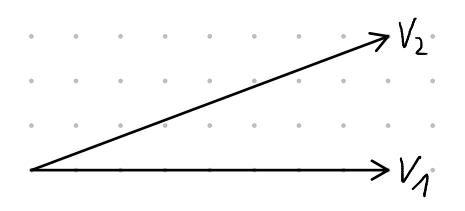
\includegraphics[width=0.25\textwidth]{Bild004}
                \caption{Problemstellung}
            \end{figure}

            $w_2=v_2-\frac{\langle v_2,v_1 \rangle_2}{\langle v_1,v_1 \rangle_2}v_1$ ist problematisch, falls $v_1\approx v_2$ (Auslöschung).
            Beim Gram-Schmidt-Verfahren können Rundungsfehler auftreten. Es ist instabil.

            \underline{\textbf{Ziel:}} Stabiler Algorithmus um $QR$-Zerlegungen zu berechnen.

        \section{Grundüberlegungen zu Orthogonalisierungsverfahren}

            \underline{\textbf{Problemstellung:}} Gegeben $v_1=\alpha e_1\in\R^2,v_2\in\R^2$ transformiere $v_2$ auf $\tilde{w_2}=\beta e_2$, gebe $\beta$ an.

            \underline{\textbf{Gram-Schmidt:}} $\beta=\left\Vert w \right\Vert_2$

            \begin{figure}[H]
                \centering
                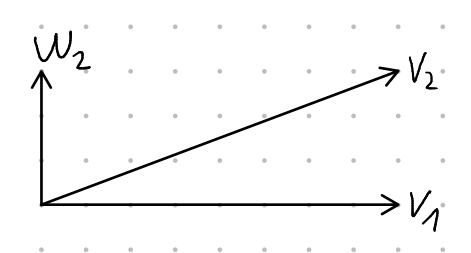
\includegraphics[width=0.25\textwidth]{Bild005}
                \caption{Gram-Schmidt}
            \end{figure}


            \underline{\textbf{Drehungen:}} $\tilde{w}_2= Qv_2$
            \[Q=\begin{bmatrix}
                \cos(-\theta) & \sin(-\theta) \\
                -\sin(-\theta) & \cos(-\theta)
            \end{bmatrix}\]
            \[\beta = \left\Vert v_2 \right\Vert_2\]

            \begin{figure}[H]
                \centering
                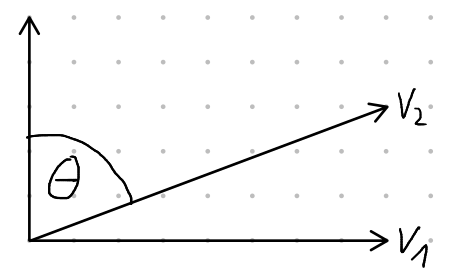
\includegraphics[width=0.25\textwidth]{Bild006}
                \caption{Drehungsansatz}
            \end{figure}


            \underline{\textbf{Spiegelungen:}} $\tilde{w}_2=Qv_2$, $Q=I-2\frac{vv^t}{v^tv}$ und $\beta=\left\Vert v_2 \right\Vert_2$

            \begin{figure}[H]
                \centering
                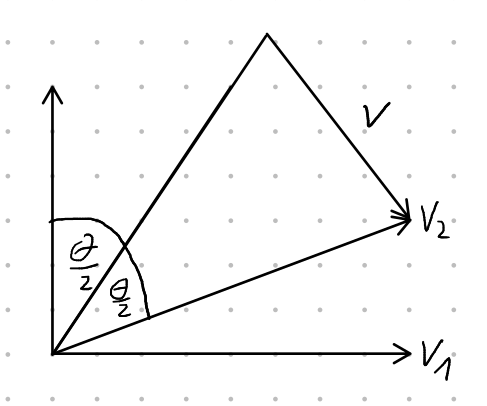
\includegraphics[width=0.25\textwidth]{Bild007}
                \caption{Spiegelungsansatz}
            \end{figure}


            \underline{\textbf{Idee:}} Benutze orthogonale Transformationen $Q_1,\dots,Q_n$ um $A\in\R^{m\times n}$ 
            ,$\rang(A)=n$, sukzessive zu reduzieren.
            \[A\rightsquigarrow Q_1A\rightsquigarrow Q_2Q_1 A\rightsquigarrow\dots\rightsquigarrow \begin{bmatrix}
                &R_1\\
                0 &\\
                \\
                & 0 &
            \end{bmatrix}\]

            Weil $\cond_2(Q)=1$ ist die Vorgehensweise stabil, bzw. gut konditioniert.

            \underline{\textbf{Aber:}} Wie wählen wir $Q_1,\dots,Q_n$?

        \section{$QR$-Zerlegung mittels Givens-Rotationen}

            \begin{definition}\label{d2.12}
                Eine Matrix der Form
                
                \[
                    \delta_{k,l}=\begin{bmatrix}
                        1 & & & & & & & & \\
                        & \ddots & & & & & & & \\
                        & & c & &  & s & & & \\
                        & & & 1 &  & & & & \\
                        & & & &  \ddots  & & & & \\
                        & & -s & & & c & & & \\
                        & &  & & & & 1 & & \\
                        & &  & & & & & \ddots & \\
                        & &  & & & & &  & 1\\
                    \end{bmatrix}
                \]
                , wobei die $s,c$ Einträge in der $k,l$ten Zeile / Spalte sind, heißen Givens-Rotationen.
            \end{definition}

            \underline{\textbf{Bemerke:}} Für $c=\cos(\theta),s=\sin(\theta)$ ist $\delta_{k,l}$ eine Drehung um $\theta$ in 
            in der Koordinaten $(k,l)$. $\delta_{k,l}$ ist Orthogonal.

            \underline{\textbf{Frage:}} Wie wählen wir $c,s$? 
            
            Gegeben $x\in\R^n$, elemeniere $l$te Koordinate zu $0$.

            \[\begin{bmatrix}
                c & s\\ -s & c
            \end{bmatrix}=\begin{bmatrix}
                x_k\\ x_l
            \end{bmatrix}=\begin{bmatrix}
                r\\0
            \end{bmatrix}\]

            \begin{figure}[H]
                \centering
                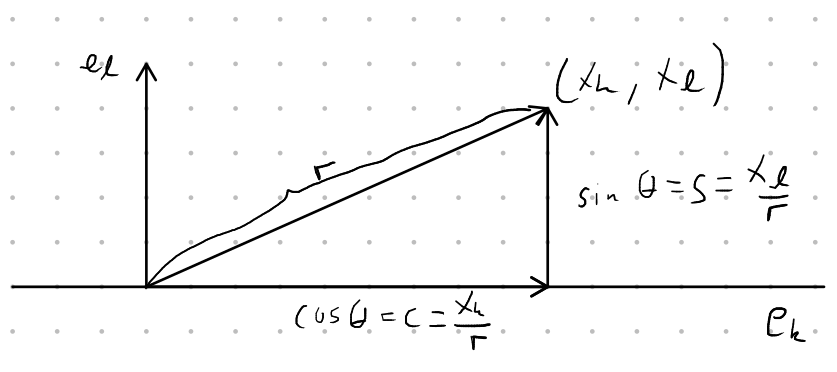
\includegraphics[width=0.25\textwidth]{Bild008}
                \caption{Trigonometriesetting}
            \end{figure}

            \begin{equation*}
                r^2=x_k^2+x_l^2
                \implies \pm \sqrt{x_k^2+x_l^2}
            \end{equation*}

            \underline{\textbf{Aber:}} Diese Berechnungsweise ist nicht unbedingt stabil ($x_k\gg x_l$)

            Stabile Variante:


            \begin{equation}\label{e2.3}
                \begin{array}{c}
                    \text{Falls }\left\vert x_l \right\vert>\left\vert x_k \right\vert\implies \tau =\frac{x_k}{x_l},s=\frac{1}{\sqrt{1+\tau^2}},c=s\tau\\
                    \text{Sonst: }\tau=\frac{x_l}{x_k},c=\frac{1}{\sqrt{1+\tau^2}},s=c\tau
                \end{array}
            \end{equation}
        

            Beispielprozess:

            \[
            \begin{bmatrix}
                * & * & * \\
                * & * & * \\
                \color{red}* & * & * \\
                \color{red}* & * & * \\
            \end{bmatrix}
            \rightsquigarrow
            \begin{bmatrix}
                * & * & * \\
                \color{red}* & * & * \\
                \color{red}* & * & * \\
                0 & * & * \\
            \end{bmatrix}
            \rightsquigarrow
            \begin{bmatrix}
                \color{red}* & * & * \\
                \color{red}* & * & * \\
                0 & * & * \\
                0 & * & * \\
            \end{bmatrix}
            \rightsquigarrow
            \begin{bmatrix}
                * & * & * \\
                0 & * & * \\
                0 & 0 & * \\
                0 & 0 & 0 \\
            \end{bmatrix}
            \]

            \begin{algorithm}[H]
                \caption{}\label{a2.13}
                \textbf{Input:} $A\in\R^{m\times n},m\geq n$\\
                \textbf{Output:} $R$ von der $QR$-Zerlegung ($A$ wird zerstört ``in place'')
                \begin{algorithmic}
                \For{$j=1,\dots, n$}
                    \For{$i=m,m-1,\dots, j+1$}
                        \State Berechne $c,s$ wie in (\ref{e2.3})
                        \State $A[i-1:i,j:n]=\begin{bmatrix}
                            c & s \\
                            -s & c 
                        \end{bmatrix}^t A[i-1:i,j:n]$
                    \EndFor
                \EndFor
                \end{algorithmic}
            \end{algorithm}

            \underline{\textbf{$m\approx n$:}}
        
            $c,s$: In jedem Eintrag einmal Wurzeln ziehen: $\implies \frac{n^2}{2}$ Quadratwurzeln und $\frac{4n^3}{3}$ Multiplikationen

            \underline{\textbf{$m\gg n$:}} $m\cdot n$ Quadratwurzeln und $2m\cdot n^2$ Multiplikationen

            \begin{remark}\label{r2.14}
                Der Algorithmus \ref{a2.13} berechnet nur $R$ von der $QR$-Zerlegung. Zur Berechnung von $Q$ müssten 
                zusätliche Operationen investiert werden um die Givens-Rotation auf $I$ anzuwenden.

                Für das lineare Ausgleichsproblem benötigen wir $Q^tb$, weshalb wir den Algorithmus auf $\left[\begin{array}{c|c}
                    A & b
                \end{array}\right]$ anwenden können (da $R=Q^t A$).
            \end{remark}

            \begin{remark}\label{b2.15}
                Für $m=n$ ist die $QR$-Zerlegung eine (teure) ALternative zur $LR$-Zerlegung.
            \end{remark}

        \section{$QR$-Zerlegung mittels Householder-Transformationen}

            \begin{definition}\label{d2.16}
                Für $v\in\R^n,v\neq 0$, heißt \[Q=I-2\frac{\overbrace{vv^t}^{\in\R^{n\times n}}}{\underbrace{v^tv}_{\in\R}}\]
                Householder-Transformation / Reflexion / Spiegelung.
            \end{definition}

            \begin{tcolorbox}[enhanced,breakable,
                title=Wichtig!]
                Nicht $vv^t$ berechnen, das ist sehr uneffizient!
            \end{tcolorbox}

            Für $a,v\in\R^n,v\neq 0$ ist $Qa=\left(I-2\frac{vv^t}{v^tv}\right)a =a-2\frac{\langle v,a \rangle_2}{\langle v,v \rangle_2}v$

            \begin{figure}[H]
                \centering
                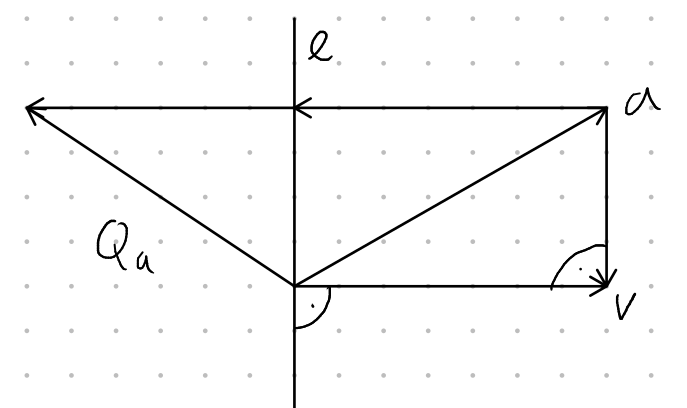
\includegraphics[width=0.25\textwidth]{Bild009}
                \caption{Householder-Transformationssetting}
            \end{figure}

            $Qa$ ist $a$ an $l$ gespiegelt.

            \begin{lemma}\label{l2.17}
                Für eine Householder-Transformation $Q\in\R^{n\times n}$ gilt:
                \begin{enumerate}
                    \item $Q$ ist symmetrisch
                    \item $Q$ ist orthogonal
                    \item $Q$ ist involutionisch (eine Involution), d.h. $Q^2=I$
                \end{enumerate}
            \end{lemma}
            \begin{proof} % TODO
                Nachrechnen.
            \end{proof}

            \underline{\textbf{Frage:}} Gegeben $a\in\R^n$, wie müssen wir $v$ wählen, so dass $Qa=\alpha e_1$ für $\alpha\in\R$?

            % TODO? Kommentar Skalarprodukt etc. schnell auf PCs

            \underline{\textbf{Beobachte:}}

            \begin{enumerate}
                \item $\left\vert \alpha \right\vert=\left\Vert \alpha e_1 \right\Vert_2 = \left\Vert Qa \right\Vert_2 = \left\Vert a \right\Vert_2$
                \item $a\underbrace{-2\frac{\langle v,a, \rangle}{\langle v,v \rangle}}_{\in\R}v=Qa$
            
                $\implies v\in\text{span}(\alpha e_1-a) \implies \alpha =\pm\left\Vert a \right\Vert_2$ % ??

                Vermeide Auslöschung $\implies \alpha=-\text{sign}(a_1)\cdot\left\Vert a \right\Vert_2$
            \end{enumerate}

            \underline{\textbf{Effiziente Berechnung:}} Beobachte:
            \begin{align*}
                \left\Vert v \right\Vert_2^2 = \langle v,v \rangle_2 &= \langle  a-\alpha e_1, a-\alpha e_1  \rangle_2&\\
                &=\left\Vert a \right\Vert_2^2-2\alpha a_1 +\alpha^2&\\
                &=-2\alpha(a_1-\alpha)&\\
                \implies Qa &= a-2\frac{\langle v,a \rangle_2}{\left\Vert v \right\Vert_2^2}=a+\frac{\langle v,a \rangle_2}{\alpha(a_1-\alpha)}v&
            \end{align*}

            \noindent
            \xrfill[0.7ex]{1pt}Ende von Vorlesung 03 am 18.10.2022\xrfill[0.7ex]{1pt}
            
            \begin{lemma}\label{l2.18}
                Sie $\alpha\in\R^n,a\neq 0,a\notin\text{span}\{e_1\}$. 
                Sei \begin{equation}\label{g2.4}
                    v=a-\alpha e_1,\alpha =-\text{sign}(a_1)\cdot \left\Vert a \right\Vert_2
                \end{equation} % oder alpha e_1-a
                Dann ist
                \begin{equation}\label{g2.5}
                    \left(I-2\frac{vv^t}{v^tv}\right)a=a+\frac{v^ta}{\alpha(a_1-\alpha)}v=\alpha e_1.
                \end{equation}
            \end{lemma}

            \begin{proof}
                Siehe oben.
            \end{proof}

            \begin{algorithm}[H]
                \caption{}\label{a2.19}
                \textbf{Input:} $A\in\R^{m\times n},m\geq n$ ``Mehr Zeilen als Spalten''\\
                \textbf{Output:} $A\in\R^{m\times n}$, obere rechte Dreiecksmatrix $R$, Rest Householder-Transformationen
                \begin{algorithmic}
                \For{$j=1,\dots, n$} \Comment Iterieren über die Spalten
                    \State Berechne $v,\alpha$ wie in (\ref{g2.4}) ,mit $a=A[j:m,j]\in\R^{m-j+1}$
                    \State $v=\frac{1}{v_1}v$ \Comment Erster Eintrag wird nicht gespeichert, daher normalisieren wir
                    \State Berechne $A[j:m,j:n]=\left(I-2\frac{vv^t}{v^tv}\right)A[j:m,j:n]$ wie in (\ref{g2.5})
                    \If{$j<m$}
                        \State A[j+1:m,j]=v[2:m-j+1]\Comment Index startet von 1 
                    \EndIf
                \EndFor
                \end{algorithmic}
            \end{algorithm}

            \begin{remark}\label{b2.20}
                Die Skalierung $v=\frac{1}{v_1}v$ stellt sicher, dass die der erste Eintrag von $v$ nicht gespeichert werden muss.
            \end{remark}

            \underline{\textbf{Aufwand:}} $m\sim n \rightsquigarrow \frac{2}{3}n^3$ Multiplikationen

            $m\gg n \rightsquigarrow 2n^2m$ Multiplikationen

            Schneller als Givensrotationen, stabiler als Normalengleichungen

        \section{Pseudoinverse}

            \underline{\textbf{Ausgangspunkt:}} Wir wollen ein stabiles numerisches Verfahren, dass 
            \[
                Ax=b,A\in\R^{m\times n},m\geq n,\rang(A)=n,b\in\R^n    
            \]
            ``lösen'' kann, d.h. es gilt 
            \[
                \left\Vert Ax-b \right\Vert_2=\min_{y\in\R^n}\left\Vert Ay-b \right\Vert_2    
            \]

            Mathematisch können wir die Abbildung $b\mapsto x$, wegen der Normalengleichung (\ref{g2.2}), schreiben als 
            \[
                x=\underbrace{(A^tA)^{-1}A^t}_{\coloneqq A^\dagger}b=A^\dagger b    
            \]
            $A^\dagger\in\R^{n\times m}$. Wegen $A^\dagger A=I$ heißt $A^\dagger$ auch \textbf{Pseudoinverse}.

            \underline{\textbf{Frage:}} Können wir den Begriff der Inversen noch weiter verallgemeinern? Auf beliebige Matrizen?

            Satz \ref{s1.9}: $A\in\R^{m\times n}, U=\text{Bild}(A)$

            \begin{align*}
                &\implies \left\Vert Ax-b \right\Vert_2=\min_{y\in\R^n} \left\Vert Ay-b \right\Vert_2 \stackrel{\text{Satz \ref{s1.9}}}{\iff} Ax-b\in\text{Bild}(A)^\perp\\
                &\iff Ax- Pb -\underbrace{(b-Pb)}_{\in U^\perp:\text{ Satz \ref{s1.9}}}\in\text{Bild}(A)^\perp, Pb \text{ ist die orthogonale Projektion von } b \text{ auf } U\\
                &\iff \underbrace{\underbrace{Ax}_{\in U}-\underbrace{Pb}_{\in U}}_{\in U}\in\text{ Bild}(A)^\perp\\
                & \iff Ax=Pb
            \end{align*}

            Falls $\rang(A)<n$ (z.B., falls $m<n$) ist $Ax=Pb$ nicht eindeutig lösbar (aber es existiert immer eine Lösung).

            Für $\tilde{x}\in\R^n$ mit $A\tilde{x}=Pb,x'\in\text{ker}(A)$ ist $A(\tilde{x}+x')=Pb$.

            \begin{align*}
                L(b)&=\left\{x\in\R^n:\left\Vert Ax-b \right\Vert_2 = \min_{y\in\R^n} \left\Vert Ay-b \right\Vert_2\right\}\\
                &=\{x\in\R^n:Ax=Pb\}\\
                &=\tilde{x}+\ker(A)
            \end{align*}

            Sind gewisse Lösungen sinnvoller als andere?

            Wähle: $x\in\tilde{x}+\ker(A)$ mit minimaler Norm als ``eindeutige'' Lösung von $Ax=b$.

            \begin{align*}
                \stackrel{\text{Bem. \ref{b1.13}}}{\implies} \left\Vert x-0 \right\Vert_2 = \min_{y\in \tilde{x}+ \ker(A)} \left\Vert y-0 \right\Vert_2 &\iff x\in (\tilde{x}+\ker(A))^\perp \\
                &\iff x\in \ker(A)^\perp 
            \end{align*}

            \begin{tcolorbox}[enhanced,breakable,
                title=Anmerkung]
                Hier ist nicht ganz klar, was mit $(\tilde{x}+\ker(A))^\perp$ gemeint ist, da dies z.B. für $\ker(A)=\text{span}\{(0,1)^t\}$ und $\tilde{x}=(1,0)^t$ nur $\{0\}$ ist, was natürlich nicht der Intuition entspricht!
                
                Statt der ursprünglichen Definition müssen wir hier wieder zurück schieben ($-\tilde{x}$ rechnen), was kein Problem ist, da wir o.B.d.A $\tilde{x}\perp \ker(A)$ vorraussetzen dürfen, bevor wir das Skalarprodukt berechnen!

                Zum Beispiel ist also $v=(1,0)^t$ im obigen Beipspiel doch im orthogonalen Komplement, da $\langle v, \tilde{x}+u-\tilde{x}\rangle_2=0$ für $u\in \ker(A)$
            \end{tcolorbox}
            
            \begin{figure}[H]
                \centering
                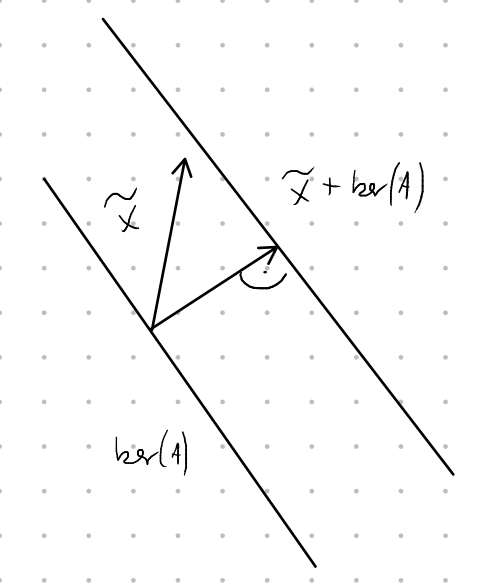
\includegraphics[width=0.25\textwidth]{Bild010}
                \caption{Setting}
            \end{figure}

            \begin{remark}\label{b2.21}
                Diese Wahl von $x$ für $b\mapsto x$ ist linear: Für $b_1,b_2\in\R^m$ ist:
                \[
                \begin{rcases*}
                Ax_1 = b_1 & $x_1 \in\text{ker}(A)^\perp$ \\
                Ax_2 = b_2 & $x_2 \in\text{ker}(A)^\perp$
                \end{rcases*} \implies P(x_1+x_2)=P(x_1)+P(x_2)=Ax_1+Ax_2=A(x_1+x_2),x_1+x_2\in \ker(A)^\perp
                \]
            \end{remark}

            \begin{definition}\label{d2.22}
                Sei $A\in\R^{m\times n}$. Die Abbildungsmatrix $A^\dagger\in\R^{n\times m}$ von $b\mapsto x$ heißt 
                \textbf{Pseudoinverse} oder \textbf{Moore-Pensore-Inverse} von $A$. D.h. gegeben $b\in\R^n$, dann ist $x=A^\dagger b$ die eindeutige Lösung von 
                \[
                    \min_{y\in\ker(A)^\perp} \left\Vert Ay-b \right\Vert_2 = \left\Vert Ax-b \right\Vert_2.    
                \]
            \end{definition}
            
            \begin{theorem}\label{s2.23}
                $A\in\R^{m\times n}$. Dann ist $A^\dagger\in\R^{m\times n}$ eindeutig über die Moore-Penrose-Axiome definiert:
                \begin{enumerate}
                    \item $(A^\dagger A)^t=AA^\dagger$
                    \item $(AA^\dagger )^t=A^\dagger A$
                    \item $A^\dagger AA^\dagger = A^\dagger$
                    \item $AA^\dagger A=A$
                \end{enumerate}
            \end{theorem}

            \begin{proof}
                Siehe Literatur oder später
            \end{proof}

            \underline{\textbf{Frage:}} Wie berechnen wir $x=A^\dagger b$?

            Sei $A\in\R^{m\times n},\rang(A)=p\leq \min(m,n)$. Bringe $A$ mittels orthogonaler Transformationen (z.B. Householder) auf 
            obere Dreiecksgestalt, d.h.:

            \begin{equation}\label{g2.6}
                Q^tA=\begin{bmatrix}
                    &  &  & & & \\
                    & R & & S & & \\
                    * & & & & &\\
                    & 0 & &  0 & & \\ 
                \end{bmatrix}
            \end{equation}
            wobei  $S\in \R^{p\times (n-p)}$.
            Setze Analog $x=\begin{bmatrix}
                x_1\in\R^p\\
                x_2\in R^{n-p}
            \end{bmatrix},Q^t b=\begin{bmatrix}
                b_1\in\R^p\\
                b_2\in \R^{m-p}
            \end{bmatrix}$

            \begin{lemma}\label{l2.24}
                Mit obigen Bezeichungen ist $x=A^\dagger b$ genau dann, wenn \[x_1=R^{-1}b_1-R^{-1}Sx_2.\]
            \end{lemma}
            \begin{proof}
                \begin{align*}
                    \left\Vert Ax-b \right\Vert_2^2&=\left\Vert Q^t(Ax-b) \right\Vert_2^2\\
                    &=\left\Vert \begin{pmatrix}
                        Rx_1+Sx_2-b\\
                        -b_2
                    \end{pmatrix} \right\Vert_2^2\\
                    &= \left\Vert Rx_1+Sx_2 -b_1\right\Vert_2^2+\left\Vert b_2 \right\Vert_2^2
                \end{align*}
                ist minimal, falls $Rx_1=b_1-Sx_2$.
            \end{proof}

            Wir sehen $p=\rang(A)=n\implies$ wie vorher, lineares Ausgleichsproblem!

            Sonst: $x_2=$?

            \begin{lemma}\label{l2.25}
                Sei $p<n,V=R^-1S\in\R^{n\times (n-p)}$ und $u=R^{-1}b_1\in\R^p$. Dann ist
                \begin{align*}
                    x&=A^\dagger b\\
                    \iff &(I+V^tV)x_2=V^tu\\
                    &x_1=u-Vx_2
                \end{align*}
            \end{lemma}

            \begin{proof}
                \begin{align*}
                    \left\Vert x \right\Vert_2^2 &= \left\Vert x_1 \right\Vert_2^2 + \left\Vert x_2 \right\Vert_2^2\\
                    &\stackrel{\text{Lemma \ref{l2.24}}}{=}\left\Vert u-Vx_2 \right\Vert_2^2+ \left\Vert x_2 \right\Vert_2^2\\
                    &=\left\Vert u \right\Vert_2^2-2 \langle u,Vx_2 \rangle_2+\langle Vx_2,Vx_2 \rangle_2+\langle x_2,x_2 \rangle_2\\
                    &=\left\Vert u \right\Vert_2^2+\langle x_2,(I+V^tV)x_2-2V^tu \rangle_2 = \varphi(x_2)
                \end{align*}
                Minimiere $\varphi(x_2)$:
                \begin{align*}
                    \varphi'(x_2)=-2V^tu+2(I+V^tV)x_2\\
                    \varphi'(x_2)=2(I+V^tV) \implies \text{spd}
                \end{align*}
                $\varphi$ minimal $\iff \varphi'(x_2)=0\implies $ Behauptung.
            \end{proof}

            \begin{algorithm}[H]
                \caption{}\label{a2.26}
                \textbf{Input:} $A\in\R^{m\times n},b\in\R^m$\\
                \textbf{Output:} $x=A^\dagger b$
                \begin{algorithmic}
                \State Berechne $QR$-Zerlegung (\ref{g2.6}) von $A$
                \State $\begin{bmatrix}b_1\\b_2\end{bmatrix}=Q^t b$
                \State $V=R^{-1}S$ mittels Rückwertssubstitution 
                \State $u=R^{-1}b_1$ mittels Rückwertssubstitution
                \State Löse $(I+V^tV)x_2=V^tu$ mittels Cholesky-Zerlegung 
                \State $x_1=u-Vx_2$
                \State $x=\begin{bmatrix}x_1\\x_2\end{bmatrix}$
                \end{algorithmic}
            \end{algorithm}

            \noindent
            \xrfill[0.7ex]{1pt}Ende von Vorlesung 04 am 20.10.2022\xrfill[0.7ex]{1pt}
            

    \chapter{Iterative Verfahren für große, dünn besetzte, Gleichungsysteme}

        \section{Motivation}

            Sei $\Omega\subset \R^d,d\in\N$. Betrachte die stationäre Wärmeleitungsgleichung, eine partielle Differenzialgleichung
            \begin{equation}\label{g3.1}
                \begin{cases}
                    -\Delta u(x)=f(x) & \in\Omega\\
                    u(x)=0 & x\in \delta\Omega
                \end{cases}
            \end{equation}

            mit Wärmequelle $f\in C(\Omega)$ und dem Laplace-Operator:

            \begin{equation}\label{g3.2}
                \Delta u =\sum_{i=1}^n \frac{\partial^2 u(x)}{\partial x_i^2}. 
            \end{equation}

            Die Lösung $u\in C^2(\Omega)$, falls existent, beschreit die Temperaturverteilung im Raum $\Omega$.

            Diese Gleichung ist i.A. nicht von Hand lösbar! 

            \underline{\textbf{Idee:}} Berechne approximative Lösung im Computer.

            \underline{\textbf{Ansatz:}} Für $g\in C^2(\R)$ ist
            \begin{align*}
                g''(x)=\lim_{h\searrow 0} \frac{g'(x+h)-g(x)}{h} &\approx \frac{g'(x+h)-g(x)}{h} \\
                & \approx \frac{\frac{g(x+h)-g(x)}{h}-\frac{g(x)-g(x-h)}{h}}{h}\\
                &\approx \frac{g(x+h)-2g(x)+g(x-h)}{h^2}
            \end{align*}

            $\rightsquigarrow$ Ersetze $\frac{\partial^2 u}{\partial x_i^2}$ in (\ref{g3.2})

            $\rightsquigarrow$ Überziehe $\Omega$ mit einem regelmäßigen Gitter mit Maschenweite $h=\frac{1}{n},n\in\N$.

            \begin{figure}[H]
                \centering
                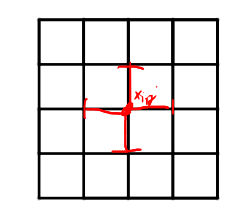
\includegraphics[width=0.25\textwidth]{Bild011}
                \caption{Gitter}
            \end{figure}

            Bezeichne die Gitterpunkte mit $x_{ij}$ und $u_{ij}=u(x_{ij})$.

            \[\stackrel{d=2}{\implies}\frac{1}{h^2}\left(4u_{ij}-u_{i+1j}-u_{i-1j}-u_{ij+1}-u_{ij-1}\right)=f_{ij}:i,j\in1,\dots,n-1\] 

            \[u_{ij}=0,i\in\{0,n\}\text{ oder }j\in\{0,n\}\]

            Wir erhalten ein lineares Gleichungssystem mit $N=(n-1)^2$ Unbekannten und $O(1)$ Einträgen pro Zeile. 
            $\implies A\in\R^{n\times n}$ hat $O(N)$ Einträge. Wir haben das Lösen eines (linearen) partiellen Differentialgleichung durch das Lösen eines linearen 
            Gleichungssystems ersetzt.

            \begin{example}\label{b3.1}
                $\Omega=(0,1)^2,n=4\implies h=\frac{1}{4}$. Erhalte:

                \[
                    \left[
                        \begin{array}{ccc|ccc|ccc}
                            4 & -1 & &-1 & & & & & \\
                            -1 & 4 & -1 & & -1 & & & & \\
                            & -1 & 4 & & & -1 & & & \\ \cline{1-9}
                            -1 & & &  4 & -1 & & -1 & & \\
                            & -1 & &  -1 & 4 & -1 & &-1 &\\
                            & & -1 & & -1 & 4 & & &  -1\\\cline{1-9}
                            & & & -1 & & & 4 & -1 & \\
                            & & & & -1 & & -1 & 4 & -1 \\
                            & & & & & -1 & & -1 & 4  
                        \end{array}  
                    \right]
                    \begin{bmatrix}
                        u_{11}\\
                        u_{12}\\
                        u_{13}\\
                        u_{21}\\
                        u_{22}\\
                        u_{23}\\
                        u_{31}\\
                        u_{32}\\
                        u_{33}
                    \end{bmatrix} = 
                    \begin{bmatrix}
                        f_{11}\\
                        f_{12}\\
                        f_{13}\\
                        f_{21}\\
                        f_{22}\\
                        f_{23}\\
                        f_{31}\\
                        f_{32}\\
                        f_{33}
                    \end{bmatrix}
                \]
            \end{example}


            \underline{\textbf{Aber:}} Um die Lösung von (\ref{g3.1}) gut zu approximierenm ist oft $N\gg 1$ erforderlich.
            Für kleine bis mittlere $N$, d.h. in 2022 je nach Modell $\sim$ 10 Millionen, sind graphenbasierte Löser eine Option.

            Was tun für große $N$?

            \underline{\textbf{Beobachtung:}} Matrix-Vektor-Multiplikation sind für dünn besetze Matrizen in $O(N)$ berechenbar.

            \underline{\textbf{Frage:}} Wie bauen wir gute Löser für LGS (lineare Gleichungssysteme) nur unter Anwendung von 
            Matrix-Vektor-Multiplikationen?

            \underline{\textbf{Idee:}} Benutze  Orthogonalität um eine Bestapproximationseigenschaft zu erhalten.

        \section{Grundidee von Projektionsmethoden}

            Sei $A\in\R^{n\times n},b\in\R^n$ und $K,L$ Unterräume vom $\R^n$.

            \underline{\textbf{Idee:}} Finde eine approximative Lösung $\tilde{x}$ zu $Ax=b$ mit 
            \[\tilde{x}\in K \text{ und } b-A\tilde{x}\perp_2 L\]
            Kanonische Wahl: $L=AK$.

            Falls wir eine Startnährung $x_0$ zu $x$ kennen, können wir $\tilde{x}$ in $x_0+K$ suchen:

            Finde $\tilde{x} \in x_0+K \text{ mit } b-A\tilde{x}\perp_2 L$

            \underline{\textbf{Beobachtung:}} $\tilde{x}\in x_0+K\implies \exists d\in K: \tilde{x}=x_0+d$

            \[\implies \underbrace{b-A(x_0}_{r}+d)\perp_2 L\]

            \[\iff r_0-Ad \perp_2 L\]

            Eine approximative Lösung $\tilde{x}=x_0+d$ muss also erfüllen:

            \begin{equation}\label{g3.3}
                \begin{cases}
                    \tilde{x}=x_0+d & \\
                    \langle r_0-Ad,w \rangle_2 = 0  & \forall w\in L
                \end{cases}
            \end{equation}

            \underline{\textbf{Idee:}} Wähle $x_0,K,L$, berechne $d\in K$ durch Lösen eines Unterproblems. Setze 
            $x_1=x_0+d$, wähle neue Unterräume, beginne von vorne.

            Wie implementieren wir diese Idee im Computer?

            Sei $K=\text{span}\{v_1, \dots, v_n\},L=\{w_1,\dots,w_n\}$

            $V=[v_1\vert \dots\vert v_n]$ und $W=[w_1\vert \dots\vert w_n]$

            (\ref{g3.3}) ist äquivalent zu 

            \begin{equation}\label{g3.4}
                \begin{cases}
                    \tilde{x} = x_0+Vy &  y\in\R^m\\
                    W_i^t A Vy = W_i^t r_0 & i=1,\dots n \iff \underbrace{W^tA}_{m\times m}Vy = W^tr_0
                \end{cases}
            \end{equation}

            $\implies \tilde{x}=x_0+V(W^tAV)^{-1}W^t r_0$ % TODO: Überprüfen

            \begin{algorithm}[H]
                \caption{Prototyp einer interativen Projektionsmethode}\label{a3.2}
                \textbf{Input:} $A\in\R^{n\times n},b\in\R^n$, Fehlertoleranz $\alpha$\\
                \textbf{Output:} Nährung $x_{i+1}\approx x$
                \begin{algorithmic}
                \State i=0
                \While {Fehlertoleranz noch nicht erreicht}
                    \State Wähle $K_i,L_i$
                    \State Wähle Basen $V,W$ von $K_i,L_i$
                    \State $r_1=Ax_i$
                    \State $y=(W^tAV)^{-1}W^tr_i$
                    \State $x_{i+1}=x_i+Vy_i$
                    \State $i=i+1$
                \EndWhile
                \end{algorithmic}
            \end{algorithm}

            \underline{\textbf{Aber:}} $W^tAV$ ist nicht notwendigerweise invertierbar:

            \begin{example}\label{b3.3}
                \[
                    A=\left[
                        \begin{array}{c|c}
                            0 & I\\\cline{1-2}
                            I & I
                        \end{array}
                    \right]\in\R^{2m\times 2m}
                \]
                \[
                    K=L=\text{span}\{e_1,\dots,e_m\}\implies V=W=\
                    \left[
                        \begin{array}{c}
                            I_m\\\cline{1-1}
                            0
                        \end{array}
                    \right]\in K^{2m\times m}
                \]
                \[\implies W^t A V =0 \text{ ist nicht invertierbar.}\]
            \end{example}

            \begin{lemma}\label{3.4}
                Sei einer der folgenden Bedingungen erfüllt:
                \begin{enumerate}
                    \item $A$ ist spd, $K=L$
                    \item $A$ invertierbar, $L=AK$
                \end{enumerate}
                Dann ist $W^tAV$ für alle Basen von $K,L$ invertierbar.
            \end{lemma}

            \begin{proof}
                \textbf{1.:} $L=K\implies W=V\delta$ mit $\delta \in R^{m\times m}$ invertierbar.

                $\implies B=W^tAV=\delta^tV^tAV$ % TODO: überprüfen

                \[0<\underbrace{y^tAy}_{=\underbrace{x^tV^t A V x}_{\text{spd, invertierbar}}},y=Vx\]

                \textbf{2.:} $L=AK \implies W=AV\delta,\delta\in\R^{m\times m}$ invertierbar

                \[\implies B=W^tAV=\delta^t\underbrace{V^tA^tAV}_{\text{spd}} \implies\text{ invertierbar } \implies \text{ Beh.}\]
            \end{proof}

            \noindent
            \xrfill[0.7ex]{1pt}Ende von Vorlesung 05 am 25.10.2022\xrfill[0.7ex]{1pt}

        \section{Verfahren des steilsten Abstiegs}

            \underline{\textbf{Idee:}} Wähle $K=L=\text{span}\{r_i\}=\text{span}\{b-Ax_i\}$

            \[\implies x_{i+1}=x_i+\underbrace{\alpha_i r_i}_{d_i\in K}\]

            \[\implies \alpha = \frac{r_i^tr_i}{r_i^tAr_i}\]
            
            \begin{algorithm}[H]
                \caption{Verfahren des steilsten Abstiegs}\label{a3.5}
                \textbf{Input:} $A,b$, Startvektor $x_0$, Fehlertoleranz\\
                \textbf{Output:} Nährung $x_{i+1}\approx x$
                \begin{algorithmic}
                \While {Fehlertoleranz noch nicht erreicht} \Comment{Praxis $\epsilon=10^{-8}$, $\left\Vert r_i \right\Vert_2<\epsilon$}
                    \State $r_i=b-Ax_i$
                    \State $\alpha_i= \frac{r_i^tr_i}{r_i^tAr_i}$
                    \State $x_{i+1}=x_i+\alpha_i r_i$
                \EndWhile
                \end{algorithmic}
            \end{algorithm}

            \begin{remark}\label{b3.6}
                Wegen (\ref{g3.3}) gilt:
                \begin{align*}
                    0&=\langle r_i-Ad_i,r_i \rangle_2\\
                    &=\langle b-Ax_i-Ad_i,r_i \rangle_2\\
                    &=\langle b-Ax_{i+1},r_i \rangle_2\\
                    &= \langle Ax-Ax_{i+1}, r_i\rangle_2\\
                    &= \langle x-x_{i+1}, r_i\rangle_A = (\star)
                \end{align*}
            \end{remark}

            Mit 
            \[
                \langle \cdot,\cdot \rangle_A=\langle A\cdot,\cdot \rangle_2
            \]

            Aus $(\star)$ folgt 

            \begin{align*}
                0=(\star) &\iff x-x_{i+1} \perp_A r_i \\
                &\iff x-x_{i+1} \perp_A x_i+\text{span}\{r_i\}\\
                &\stackrel{\text{Satz \ref*{s1.9}}}{\iff} \left\Vert x-x_{i+1} \right\Vert_A=\min_{y\in x_i+\text{span}\{r_i\}} \left\Vert x-y \right\Vert_A\\
                &\iff \frac{1}{2} \left\Vert x-x_{i+1}  \right\Vert_A^2 = \min_{\alpha\in \R}=\frac{1}{2} \left\Vert  x-x_i-\alpha r_i \right\Vert_A^2
            \end{align*}

            Betrachte $f(x_i)=\frac{1}{2}\left\Vert x-x_i \right\Vert_A^2 = \frac{1}{2} \langle A(x-x_i),x-x_i \rangle_2$

            \[
                f'(x_i)=-\underbrace{Ax}_{=b}+Ax_i=-r_i    
            \]

            D.h. am Punkt $x_i$ gehen wir in Richtung des steilsten Abstiegs,

            \begin{theorem}\label{s3.7}
                Sei $A\in\R^{n\times n}$ spd. Dann gilt für die Iterierung des Verfahrens des steilsten Abstiegsm dass:
                \begin{align*}
                    \left\Vert x-x_{i+1} \right\Vert_A &\leq \frac{\lambda_{\max}(A)-\lambda_{\min}(A)}{\lambda_{\max}(A)+\lambda_{\min}(A)} \left\Vert x-x_i \right\Vert_A\\
                    &\stackrel{\frac{1}{\lambda_{\min}}}{=}\frac{\cond_2(A)-1}{\cond_2(A)+1}\left\Vert x-x_i \right\Vert_A
                \end{align*}
                wobei $\lambda_{\max},\lambda_{\min}$ die größten, kleinsten Eigenwerte sind.
            \end{theorem}

            \begin{proof}
                Übung %TODO
            \end{proof}

            \begin{remark}\label{b3.8}
                Im Prinzip lassen sich mit Hilfe der Normalengleichung auch allgemeinere (invertierbare) Matrizen behandeln. 
                Hierbei wird die Kondition verschlechtetertm d.h. die Konvergenz verschlechtert sich.
            \end{remark}

        \section{Krylovräume}

            \underline{\textbf{Beobachte:}} Im Verfahren des steilsten Abstiegs gilt:
            \[
                x_i=x_0+\alpha_0r_0+\dots+\alpha_{i-1}r_{i-1} = x_0+\alpha_0r_0+\dots+(\alpha_{i-2}I+\alpha_{i-1}(I-\alpha_{i-2}))r_{i-2}
            \]
            \[=x_0 q_{i-1}(A)r_0, q_{i-1}\in\Pi_{i-1}\]

            \underline{\textbf{Idee:}} Finde eine bessere Approximation von $x_i$ in $x_0+K_{i-1}(A,r_0)$.

            \begin{definition}\label{d3.9}
                Sei $A\in\R^{n\times n},v\in\R^n,n\geq 1$. Der Raum 
                \[K_m=\text{span}(v,Av,A^2v,\dots,A^{m-1}v)\]
                heißt \textbf{Kylovraum} von $A$ zu $v$.                
            \end{definition}

            Es gilt $K_m(A,v)\subseteq K_{m+1}(A,v)$

            \begin{lemma}\label{l3.10}
                Sei $\R^{n\times n},v\in\R^n$. Dann gilt:
                \begin{enumerate}
                    \item $\dim K_m(A,v)\leq \min\{m,n\}$
                    \item $\dim(K_m(A,v))=\dim(K_{m+1}(A,v))=m\implies \dim(K_{m+i}(A,v))=m,i=0,1,\dots$
                    \item Für $m$ wie im 2. gilt \[\{Ax:x\in K_m(A,v)\}\subseteq K_m(A,v)\]
                    D.h. $K_m(A,v)$ ist invariant unter $A$.
                \end{enumerate}
            \end{lemma}

            \begin{proof}
                Übung   
            \end{proof}

            \begin{remark}\label{b3.11}
                Betrachte $Ax=b$ mit Startnährung $x_0$, Residuum $r_0=b-Ax_0$. Für $i=0,\dots$. Wähle
                \[x_{i+1}\in x_0+K_{i-1}(A,r_0)\]
                \[\implies x_{i+1}x_0=q_i(A)r_0\]
                \[\implies r_{i+1}=b-Ax_{i+1}=\underbrace{b-Ax_0}_{r_0}-Aq_i(A)r_0\]
                \[=q_{i+1}(A)r_0\in K_{i+2}(A,r_0)\]
            \end{remark}

            \underline{\textbf{Das bedeutet:}} Sind $K,L$ geeignete Krylovräume in einer Projektionsmethode, dann können 
            wwir immer garantieren, dass das Ergebnis in einem Krylovraum ist.

            \underline{\textbf{Aber:}} Die Vektoren $v,Av,\dots,A^nv$ sind numerisch keine guten Basen der Krylovräume, da sie zunehmend in eine 
            änhliche Richtung zeigen.

        \section{Arnoldi-Verfahren}

            \underline{\textbf{Gesucht:}} Numerisch gutartige Basis von $K_m(A,v)$, welche einfach zu einer gutartigen Basis von $K_{m+1}(A,v)$ erweitert werden kann.

            \underline{\textbf{Idee:}} Arrangiere die Vektoren $v,Av,\dots$ in einer ``wachsenden'' Matrix
            \[[v\vert Av\vert A^2v\vert \dots]\]
            und wende auf jede Spalte ein Orthogonalisierungsverfahren (Gram-Schmidt, Householder,Givens) an.

            \begin{algorithm}[H]
                \caption{Arnoldi-Verfahren (Gram-Schmidt Variante)}\label{a3.12}
                \textbf{Input:} $A\in\R^{n\times n},b\in\R^n,m\in\N$\\
                \textbf{Output:} $V_m=[v_1\vert \dots\vert v_m]$ ONB von $K_m(A,v),v_{m+1}\in\R^n,H_{m+1,m}\in\R^{(m+1)\times m}$
                \begin{algorithmic}
                \State $v_1=\frac{v}{\left\Vert v \right\Vert_2}$
                \For{$j=1,m$}
                    \State $z=Av_j$ \Comment $\neq A^{j-1}r_0$
                    \State $h_{ij}=\langle z,v_i \rangle_2,i=1,\dots j$
                    \State $w_j=z-\sum_{i=1}^j h_{ij}v_i$
                    \State $h_{j+1,j}=\left\Vert w_j \right\Vert_2$
                    \If{$h_{j+1,j}=0$} 
                        \State stop \Comment Krylovraum stagniert
                    \EndIf
                \State $v_{j+1}=\frac{w_j}{h_{j+1,j}}$
                \EndFor
                \end{algorithmic}
            \end{algorithm}

            \noindent
            \xrfill[0.7ex]{1pt}Ende von Vorlesung 06 am 27.10.2022\xrfill[0.7ex]{1pt}

            \begin{lemma}\label{l3.13}
                Falls das Arnoldi-Verfahren nicht vorzeitig abbricht, ist $v_1,\dots,v_m$ eine 
                ONB von $K_m(A,r_0)$.
            \end{lemma}
            \begin{proof}
                Orthogonalität: Ok

                Orthonormal: Ok

                Basis von $K_m(A,r_0)$: $j=1$ ok

                $j\implies j+1$

                $h_{j+1,j}v_j = w_j$ (folgt aus der letzten Zeile von Algorithmus \ref{a3.12}).
                \[
                    w_j=\underbrace{Av_j}_{\in K_j(A,r_0)\implies v_j=q_{j-1}(A)v}-\underbrace{\sum_{i=1}^2h_{i,j}v_i}_{\tilde{q}_{j-1}(A)v, \tilde{q}_{j-1}\in \Pi_{j-1}}  = (\star)
                \]
                \[
                    (\star) = Aq_{j-1}(A)v_j - \tilde{q}_{j-1}(A)v_j=\underbrace{q_{j}(A)v}_{\in K_{j+1}(A,r_0)}    
                \]
            \end{proof}

            \underline{\textbf{Bemerke:}} Diese Matrix $H_{h+1,j}\in\R^{(j+1)\times j}$ hat eine bestimmte Sturktur,
            die Hessenberg-Struktur genannt wird.

            \begin{tcolorbox}[enhanced,breakable,
                title=Vorteile dieser Struktur]
                Zum Beipspiel kann man eine $QR$-Zerlegung finden, in dem man Pro Spalte eome Givensrotation anwendet.
            \end{tcolorbox}

            \begin{lemma}\label{l3.14}
                Seien $V_m\in\R^{n\times n}, H_{m+1,m}\in\R^{(m+1)\times m}$, wie im Arnoldi-Verfahren erzeugt. Sei $H_{m,m}\in\R^{m\times m}$ wie $H_{m+1,m}$, aber 
                ohne die letzte Zeile. Dann gilt:
                \begin{equation}\label{g3.5}
                    \underbrace{A}_{\in \R^{n\times n}}\underbrace{V_m}_{\in \R^{n\times m}}=\underbrace{V_m}_{\in \R^{n\times m}}\underbrace{H_{m,m}}_{\in \R^{m\times m}}+\underbrace{w_me_m^t}_{\in \R^{m\times m}}=\underbrace{V_{m+1}}_{\in \R^{n\times m+1}}\underbrace{H_{m+1,m}}_{\in \R^{m+1\times m}}
                \end{equation}
                
                \begin{equation}\label{g3.6}
                    V_m^tAV_m=H_{m,m}
                \end{equation}

            \end{lemma}

            \begin{proof}
                Gemäß Algorithmus haben wir 
                \[
                    Av_j=z=\underbrace{w_j}_{h_{j+1,j}v_j} + \sum_{i=1}^{j}h_{ij} v_i = \sum_{i=1}^{j+1} h_{ij} v_i : j=1,\dots, m    
                \]
                Daher gilt (\ref{g3.5}) (folgt aus Matrix Schreibweise).

                Für (\ref{g3.6}):

                \[
                    V_m^t A V_m = \underbrace{V^t_m V_m}_{=I} H_{m,m}+ \underbrace{V_m^t w_m e_m^t}_{=0} = H_{m,m} 
                \]
            \end{proof}

            \begin{lemma}\label{l3.15}
                Sei $j$ der Iterationsindex, bei dem das Arnoldi-Verfahren das erste Mal abbricht. Dann gilt:

                \[
                  K_j(A,r_0)=\dots = K_m(A,r_0)  
                \]
                \[
                  AV_m=V_m H_{m,m}  
                \]
            \end{lemma}

            \begin{proof}
                Übung.
            \end{proof}

        \section{Verfahren der vollständigen Orthogonalisierung}

            \underline{\textbf{Ziel:}} Kombinieren von unserem Wissen über Projektionsmethoden mit demjenigen 
            Wissen über Krylovräume.

            \underline{\textbf{Zutaten:}}
            \begin{itemize}
                \item Finde $\tilde{x}\in x_0+K$ s.d. $bA\tilde{x}\perp L$
                \item Wähle $K,L$ als Krylovräume in jeder Iteration
                \item Wähle Basen $V,W$ von $K,L$ in jeder Iteration
            \end{itemize}

            \[
                (\ref{g3.4}) \implies \begin{cases}
                    \tilde{x}=x_0+Vy\\
                    W^t A Vy = w^tr_0
                \end{cases}    
            \]

            \underline{\textbf{Idee:}} Setze $r_0=b-Ax_0,K=L=K_m(A,r_0)$ im $m$-ter Iteration, 
            $V=W$ ONB von $K_m(A,r_0)$, berechnet mittels Arnoldi-Verfahren.   

            \underline{\textbf{Zutaten: aktualisiert}}:
            \begin{itemize}
                \item $r_0=b-Ax_0$
                \item $\beta=\left\Vert r_0 \right\Vert_2,v_1=\frac{r_0}{\beta}$
                \item \[
                  \begin{cases}
                    x_m=x_0+V_my_m\\
                    \underbrace{V_m^t AV_m}_{\stackrel{\ref{g3.6}}{=}H_{m,m}}\underbrace{y_m}_{\beta v_1} = V_m^t r_0 \iff H_{m,m}y_m=\beta e_1
                  \end{cases}  
                \]
            \end{itemize}

            \begin{algorithm}[H]
                \caption{Verfahren der vollständigen Orthogonalisierung}\label{a3.16}
                \textbf{Input:} $A\in\R^{n\times n},b\in\R^n,x_0\in\R^n,m\in\N$\\
                \textbf{Output:} $x_m\in x_0+K_m(A,r_0),b-Ax_m\perp K_m(A,r_0), x_m\approx A^{-1}b$
                \begin{algorithmic}
                \State $r_0=b-Ax_0,\beta=\left\Vert r_0 \right\Vert_2,v_1=\frac{r_0}{\beta}$
                \For{$j=1,m$}
                    \State Bestimme $V_j, H_{j,j}$ mit Arnoldi-Verfahren (Stop beim Abbruch)
                    \State Löse $\underbrace{H_{j,j}}_{\in\R^{j\times j}}y_j = \beta e_1$
                    \State $x_j=x_0+V_jy_j$
                    \State Konvergenztest
                \EndFor
                \end{algorithmic}
            \end{algorithm}

            Was ist ein geeigneter Konvergenztest?

            \begin{lemma}\label{l3.17}
                Im Algorihtmus \ref{a3.16} gilt 
                \[r_m=b-Ax_m=-h_{m+1,m}(e_m^ty_m)V_{m+1}\]
                d.h. es gilt auch 
                \[
                    \left\Vert r_m \right\Vert_2 = \vert \underbrace{h_{m+1,m}}_{>0} (e^t_m y_m)\vert = h_{m+1,m} \left\vert e_m^ty_m \right\vert    
                \]
            \end{lemma}

            \begin{proof}
                \begin{align*}
                    b-Ax_m&=b-A(x_0+V_my_m)\\
                    &= r_0-  AV_my_m = (\star)
                \end{align*}
                \begin{align*}
                    (\star)&= \underbrace{r_0}_{\beta v_1}-\underbrace{AV_m}_{\stackrel{\ref{g3.5}}{=}V_mH_{m,m}-w_me_m^t}\\
                     &= \beta v_1 - \underbrace{V_m\underbrace{H_{m,m}y_m}_{=\beta e_1}}_{\beta v_1}- \underbrace{w_m}_{=h_{m+1,m}V_{m+1}}(e_m^ty_m)\\
                     &= -h_{m+1,m}(e_m^ty_m)v_{m+1}
                \end{align*}
            \end{proof}

            \underline{\textbf{Bemerke:}}

                \begin{itemize}
                    \item Hauptkosten (Alles mit Vektoren der Länge \underline{$n$})
                        \begin{itemize}
                            \item Matrix-Vektor-Multiplikation (1, Mal, sehr teuer)
                            \item Skalarprodukte
                            \item Vektor-Updates
                        \end{itemize}
                    $\implies$ Berechnen des Residuums wie in Lemma (\ref{l3.17}) lohnt sich.
                    \item Speicherbedarf und Aufwand per Iteration werden in jeder Iteration teuer!
                \end{itemize}

            \begin{tcolorbox}[enhanced,breakable,
                title=Umgehen von großen $m$]
                Wir können Neustarten, um $m$ wieder auf $1$ zu setzen und hohe Kosten von großen $m$ zu verhindern.
            \end{tcolorbox}

            \noindent
            \xrfill[0.7ex]{1pt}Ende von Vorlesung 07 am 03.11.2022\xrfill[0.7ex]{1pt}

        \section{Das GMRES-Verfahren}

            \underline{\textbf{Idee:}} Lemma (\ref{l3.17}) gibt uns eine explizite Darstellung
            von $\left\Vert r_j \right\Vert_2$. Können wir die Idee dahinter benutzen, um $\left\Vert r_j \right\Vert_2$
            in jeder Iteration zu minimieren?


            \begin{align*}
                r_j&=b-A\underbrace{x_j}_{=x_0+V_jy_j}\\
                &= \underbrace{b-Ax_0}_{=r_0=\beta v_1=V_{m+1}\beta \underbrace{e_1}_{\in\R^{m+1}}}-\underbrace{AV_j}_{\stackrel{\ref{g3.5}}{=}V_{j+1}H_{j+1,j}}y_j\\
                &= V_{j+1}(\beta e_1-H_{j+1,j}y_j)
            \end{align*}

            \[\implies \left\Vert r_j \right\Vert_2=\left\Vert V_{j+1}(\beta e_1-H_{j+1,j}y_j) \right\Vert_2\]
            
            Da $ \left\Vert V_{j+1}z_{j+1} \right\Vert_2^2=z_{j+1}^tz_{j+1}=\left\Vert z_{j+1} \right\Vert_2^2$


            \begin{equation}\label{g3.7}
                \implies \left\Vert r_j \right\Vert_2=\left\Vert \underbrace{\beta e_1}_{\in\R^{j+1}} - \underbrace{H_{j+1,j}}_{\in\R^{j+1\times j}}\underbrace{y_j}_{\in\R^{j}} \right\Vert  
            \end{equation}
            
            $\implies \left\Vert r_j \right\Vert_2$ wird minimal, falls $y_j$ als Lösung des linaren Ausgleichsproblems 
            $H_{j+1,j}y_j=\beta e_1$ gewählt wird.

            \begin{algorithm}[H] % Vllt. auch 3.18?
                \caption{GMRES-Verfahren, Generalized Minimal Residual Method, Prototyp}\label{a3.18}
                \textbf{Input:} $A\in\R^{n\times n},b\in\R^n,x_0\in\R^n,m\in\N$\\
                \textbf{Output:} $x_m\in x_0+K_m(A,r_0),\left\Vert r_m \right\Vert_2=\left\Vert b-Ax_m \right\Vert_2$ minimal
                \begin{algorithmic}
                \State $r_0=b-Ax_0,\beta=\left\Vert r_0 \right\Vert_2,v_1=\frac{r_0}{\beta}$
                \For{$j=1,m$}
                    \State Bestimme $V_{j+1}, H_{j+1,j}$ mit Arnoldi-Verfahren (Stop beim Abbruch)
                    \State Löse $H_{j+1,j}y_j=\beta e_1$
                    \State $x_j=x_0+V_jy_j$
                    \State Konvergenztest
                \EndFor
                \end{algorithmic}
            \end{algorithm}

            \begin{remark}\label{b3.19} % vllt. 3.19
                \begin{enumerate}
                    \item Bis auf die Minimalitätseigenschaft von $\left\Vert r_j \right\Vert_2$ stimmen die Algotihmen \ref{a3.16} und \ref{a3.18} weitgehen überein.
                    D.h. sie haben auch ähnliche Nachteile.
                \item Algorithmus \ref{a3.18} kann auch als Projektionsmethode mit $K=K_m(A,r_0)$ und 
                      $L=AK$ hergeleitet werden. (2 Zeiler, wenn man die richtige Formel sieht)
                \end{enumerate}
            \end{remark}

            \underline{\textbf{Frage:}} wie können wir den Algortihmus \ref{a3.18} praxistauglich machen.
            D.h.: Was ist ein geeigneter Konvergenztest und wie lösen wir das lineare Ausgleichsproblem?

            \underline{\textbf{Beobachte:}} ()\ref{g3.7}) sagt: $\left\Vert r_j \right\Vert_2$ ist genau der Fehler des linearen 
            Ausgleichsproblems. Diesen Fehler können wir explizit berechnen!

            Analog zum Beweis von Satz \ref{s2.11}:

            Sei \(H_{j+1,j}=Q_jR_j=\underbrace{Q_j}_{\in\R^{j+1,j+1}}\begin{bmatrix}
                R_j\\\underbrace{0}_{\in\R}
            \end{bmatrix}\) eine QR-Zerlegung.

            Sei 
            \[
                Q^t\beta e_1 = \begin{bmatrix}
                    \overbrace{b_1}^{\in\R^j}\\\underbrace{b_2}_{\in\R}
                \end{bmatrix}
            \]

            \[
                \left\Vert r_j \right\Vert_2^2 \stackrel{(\ref{g3.7})}{=} \left\Vert \beta e_1- H_{j+1,j}y_j \right\Vert_2^2 = \left\Vert  Q^t(\beta e_1- H_{j+1,j}y_j)  \right\Vert_2^2 = (\star)
            \]

            
            \[
                (\star) = \left\Vert \begin{pmatrix}
                    b_1-\tilde{R}_jy_j\\
                    b_2
                \end{pmatrix} \right\Vert_2^2    
            \]

            \[
                = \underbrace{\left\Vert  b_1-\tilde{R}_jy_j\right\Vert_2^2}_{=0\text{ falls $H_{j+1,j}$ bzw. $\tilde{R}_j$ vollen Rang hat}} + \underbrace{\left\Vert b_2 \right\Vert_2^2}_{=\vert b \vert^2} 
            \]
             
            \[
                \implies \left\Vert r_j \right\Vert_2 = \left\vert b_2 \right\vert    
            \]  

            Wir berechnen $b_2$ als Nebenprodukt beim Lösen des linearen Ausgleichsrpoblems.

            \underline{\textbf{Aber:}} In jeder Iteration eine QR-Zerlegung zu berechnen ist teuer. Wie geht es besser?

            \underline{\textbf{Beobachte:}} \begin{itemize}
                \item $H_{j+1,j}$ hat Hessenbergstruktur, d.h. \(H_{j+1,j}\) hat Ist eine rechte obere Dreiecksmatrix, wo zusätzlich die utere Diagonale nicht notwendigerweise 0 ist. 
                Dafür kann mit $j$ Givensrotaionen eine QR-Zerlegung berechnet werden.
                \item Beim Iterationsschritt $j\implies j+1$ werden jediglich eine neue Spalte und eine neue Zeile an $H_{j+1,j}$ drangehängt um 
                um $H_{j+2,j+1}$ zu erhalten. Die restlichen Einträge bleiben unverändert.
            \end{itemize}

            Sei $H_{j+1,j}=Q_jR_j$ eine QR-Zerlegung.

            \begin{equation*}
                \begin{bmatrix}Q_j^t & 0\\ 0 & 1\end{bmatrix} H_{j+2,j+1} = 
                \begin{bmatrix}Q_j^t & 0\\ 0 & 1\end{bmatrix} \begin{bmatrix}H_{j+1,j} & \star\\ 0 & \star \end{bmatrix} =
            \end{equation*}

            % Matrix einfügen

            Die letzte Matrix kann mittels einer einzigen Givensrotation in obere Dreiecksgestalt gebracht werden.

            $\implies$ Erweitere QR-Zerlegung iin jedem Schrit.

            \noindent
            \xrfill[0.7ex]{1pt}Ende von Vorlesung 08 am 08.11.2022\xrfill[0.7ex]{1pt}
            
            \begin{algorithm}[H] % Vllt. auch 3.18?
                \caption{GMRES}\label{a3.20}
                \textbf{Input:} $A\in\R^{n\times n},b\in\R^n,x_0\in\R^n,m\in\N$\\
                \textbf{Output:} $x_m\in x_0+K_m(A,r_0),\left\Vert r_m \right\Vert_2=\left\Vert b-Ax_m \right\Vert_2$ minimal
                \begin{algorithmic}
                \State $r_0=b-Ax_0,\beta=\left\Vert r_0 \right\Vert_2,v_1=\frac{r_0}{\beta}$
                \State $\hat{b}=\beta e_1$
                \For{$j=1,m$}
                    \State Bestimme $V_{j+1}, H_{j+1,j}$ mit Arnoldi-Verfahren \Comment Durch Anhängen von Spalten/ Zeilen, Stop beim Abbruch
                    \State Wende $G_{12},G_{23},\dots,G_{j-1,j}$ auf die letzte Spalte von $H_{j+1,j}$ an
                    \State Bestimme $G_{j,j+1}$ so, dass $H_{h+1,j}=G_{j,j+1}H_{j+1,j}=\begin{bmatrix}
                        \tilde{R}_{j+1}\\0
                    \end{bmatrix}$
                    \State $\hat{b}=G_{j,j+1}\hat{b}$
                    \If{$\hat{b}$ klein}
                        \State Löse $\tilde{R}_jy_j = [\hat{b}_i]_{i=1,\dots,j}$
                        \State Gebe $x_j=x_0+V_jy_j$ zurück
                    \EndIf
                \EndFor
                \State Berechne $x_m$ wie oben, beginne von vorne mit $x_0=x_m$
                \end{algorithmic}
            \end{algorithm}

            \begin{remark}\label{b3.21}
                \begin{enumerate}
                    \item Außer, dass GMRES für invertierte Matrizen für $m=n$ konvergiert,
                    ist bis heute wenig über Konvergenzaussagen bekannt.
                    \item Außer der Matrix-Vektor-Multiplikation im Arnoldi-Verfahren sind an der j-ten Iteration 
                    nur Vektor/ Matrizen der größe $~j$, bzw. $~j\times j$ beteiligt.
                    Der Lösungsvektor wird erst nach erfülltem Konvergenzkriterium zusammengesetzt.
                    \item Für $m\ll n$ sprechen wir von einem \textbf{Restarted-GMRES}. Oft ist z.B. $m=20$
                    ausreichend.
                    \item Das Verfahren der vollständigen Orthogonalisierung kann analog abgeändert werden.
                    \item Falls das Arnoldi-Verfahren abbricht, ist die Nährungslösung exakt (``Lucky Breakdown'', Übung).
                    \item Das GMRES-Verfahren ist heutzutage (2022) eines der beliebtesten Verfahren zum Lösen LGS ohne
                    weitere, besondere Eigenschaften.
                \end{enumerate}
            \end{remark}

        \section{Der symmetrische Lanczos-Prozess}

            \underline{\textbf{Frage:}} Können wir ein besseres Verfahren herleiten, wenn wir zusäztliche
            Annahmen zu unserer Matrix treffen?
            z.B. Symmetrie oder spd?

            \underline{\textbf{Beobachte:}} Für $A$ symmetrisch ist 
            \begin{equation*}
                H_{m,m} \stackrel{(\ref{g3.6})}{=} V_m^t A V_m
            \end{equation*}
            symmetrisch und hat Hessenberg-Struktur 
            \begin{equation*}
                H_{m,m}=\begin{bmatrix}
                    \alpha_1 & \beta_1 & & & & \\
                    \beta_1 & \alpha_2 & & & & \\
                     & \beta_2 & \ddots & \ddots&  & \\
                     &  & \ddots & \ddots & \ddots  & \\
                     &  & & \beta_{n-1} & \alpha_{n-1} & \beta_{n-1}\\
                     &  & & & \beta_n & \alpha_n 
                \end{bmatrix}
            \end{equation*} 

            Die vom Arnoldi-Verfahren generierte Matrix $T_m=H_{m,m}$ ist tridiagonal und symmetrisch.
            \underline{\textbf{Idee:}} 
            \begin{itemize}
                \item Die null-Einträge $h_{ij}=\langle v_j,v_i \rangle, i=1,\dots j-2$ müssen gar nicht erst berechnet werden
                \item Wir können die Synmmetrie im Algorithmus explizit ausnutzen.
            \end{itemize}
            
            \begin{algorithm}[H] % Vllt. auch 3.18?
                \caption{Lanczos-Verfahren}\label{a3.22}
                \textbf{Input:} $A\in\R^{n\times n}$ symmetrisch, $v\in\R^n,x_0\in\R^n,m\in\N$\\
                \textbf{Output:} $V_m=\begin{bmatrix}
                    v_1 & \dots v_m
                \end{bmatrix}$ von $K_m(A,v), v_{m+1}\in\R^n,\beta\in\R,T_m\in\R^{m\times m}$
                \begin{algorithmic}
                \State $\beta_1=0,v_0=0$
                \For{$j=1,m$}
                    \State $h_{ij}=0,i=1,\dots,j_2$
                    \State $h_{j-1,j}=\beta_j$
                    \State $w_j=z-\sum_{i=1}^{j-1}h_{ij}v_i=Av_j-\beta_jv_{j-1}$ \Comment In der Praxis hat $w$ keinen Index
                    \State $\alpha_j = \langle w_j, v_j\rangle_2=h_{jj}$
                    \State $w_j=w_j-\alpha_j v_j$ \Comment $w=Av_j-\alpha_jv_j-\beta_jv_{j-1}$
                    \State $\beta_{j+1}=\left\Vert w_j \right\Vert_2$
                    \If{$\beta_{j+1}=0$} \Comment in der Praxis: testen ob Betrag klein
                        \State Stop  
                    \EndIf
                    $v_{j+1}=\frac{w_j}{\beta_{j+1}}$
                \EndFor
                \State Berechne $x_m$ wie oben, beginne von vorne mit $x_0=x_m$
                \end{algorithmic}
            \end{algorithm}

            \begin{remark}\label{b3.23}
                Das Lanczos-Verfahren implementiert die Berechnung der ONB als Drei-Term-Rekursion,
                die für höhere Iterationszahlen instabil werden kann.
            \end{remark}

            \underline{\textbf{Idee:}} Wende unser neues Verfahren auf die Methode der vollständigen
            Orthogonalisierung an.

            \begin{algorithm}[H] % Vllt. auch 3.18?
                \caption{Lanczos-Verfahren für lineare GLeichungssysteme}\label{a3.24}
                \textbf{Input:} $A\in\R^{n\times n}$ symmetrisch, $b\in\R^n,x_0\in\R^n,m\in\N$\\
                \textbf{Output:} $x_m\in x_0 +K_m(A,r_0), x_m\approx A^{-1}b$
                \begin{algorithmic}
                \State $r_0=b-Ax_0,\beta=\left\Vert r_0 \right\Vert_2,v_1=\frac{r_0}{\beta_1}$
                \For{$j=1,m$}
                    \State Bestimme $V_j,T_j$ mittel Lanczos-Verfahren (Stop bei Abbruch)
                    \State Löse $T_jy_j = \beta e_1$
                    \State $x_j =x_0 V_jy_j$
                    \State Konvergenztest
                \EndFor
                \State Berechne $x_m$ wie oben, beginne von vorne mit $x_0=x_m$
                \end{algorithmic}
            \end{algorithm}

            \begin{remark}\label{b3.25}
                \begin{enumerate}
                    \item Lemma \ref{l3.17}, d.h. 
                    \[\left\Vert r_j \right\Vert_2=\left\Vert b-Ax_j \right\Vert_2=\beta_{j+1}\left\vert e_j^ty_j \right\vert\]
                    gilt weiterhin. Wir können den Konvergenztest also ohne Berechnung von $x_j$ durchführen.
                    \item Da $T_j$ tridiagonal ist, kann $T_jy_j=\beta e_1$ in $O(j)$ gelöst werden.
                    \item Speicherbedarf und Rechenaufwand wachsen immer noch mit $j$. 
                \end{enumerate}
            \end{remark}

            \noindent
            \xrfill[0.7ex]{1pt}Ende von Vorlesung 09 am 10.11.2022\xrfill[0.7ex]{1pt}
            
            \underline{\textbf{Frage:}}  Können wir es vermeiden die Basis $V_j$ vom Krylovraum 
            zu speichern?

            \underline{\textbf{Beobachte:}} Betrachte $LR$-zerlegung
            \begin{equation*}
                T_m=L_mR_m = \begin{pmatrix}
                    1 & & &\\
                    \lambda_2 & \ddots & & \\
                    & \ddots & \ddots &\\
                    && \lambda_m & 1
                \end{pmatrix}
                \begin{pmatrix}
                    \eta_1 & \beta_2& &\\
                     & \ddots & \ddots& \\
                    && \ddots & \beta_m \\
                    &&  & \eta_m
                \end{pmatrix}
            \end{equation*}

            Zeile und Spalte ergänzen:
            \[\lambda_m=\frac{\beta_m}{\eta_{m+1}}, \eta_m = \alpha_m -\lambda_m\beta_m\]

            Wobei $\alpha_i$ die Einträge auf der Diagonalen und $\beta_j$ die Einträge der Nebendiagonalen von $T_j$ sind.

            \[\implies x_m= x_0 + \underbrace{V_my_m}_{T^{-1}_m\beta e_1=R^{-1}_mL^{-1}_m \beta e_1}\]
            \[x_0=\underbrace{V_mR^{-1}_m}_{P_m}\underbrace{L^{-1}_m\beta e_1}_{z_m}\]

            \[P_mR_m=V_m\implies v_m=\beta_m p_{m-1}+\eta_m p_m\]
            \[\implies p_m=\frac{1}{2}(v_m-\beta_m p_{m-1})\]

            D.h. $P_m$ kann mit wachsendem $m$ einfach und effizient berechnet werden.

            % Falsch
            \[z_m=L_m^{-1}\beta e_1=\begin{pmatrix}
                &  &&& \textbf{0}\\
                & &L_{m-1}^{-1}& & \vdots\\
                &  & &&\textbf{0}\\
                0 & \dots & 0 & -\lambda_m & 1
            \end{pmatrix}
            \begin{pmatrix}
                \beta \\
                \\
                \\
                \\
                0
            \end{pmatrix}
            =\begin{pmatrix}
                \\
                \\
                z_{m-1}
                \\
                \\
                \zeta_m 
            \end{pmatrix}\]
            %Falsch Ende 
            \[\begin{bmatrix}
                &  &&& \\
                & &L_{m-1}^{-1}& &\\
                &  & &&\\
                0 & \dots & 0 & -\lambda_m & 1
            \end{bmatrix}\begin{bmatrix}
                \\
                \\
                z_{m-1}
                \\
                \\
                \zeta_m 
            \end{bmatrix}=L_mz_m=\beta e_1 = \begin{bmatrix}
                \beta \\
                0\\
                \vdots\\
                0
            \end{bmatrix}\]
            Mit $\zeta_m=-\lambda_m \zeta_{m-1}$

            \begin{align*}
                \implies x_m&=x_o+p_mz_m\\
                &= x_0 + \begin{bmatrix}
                    p_{m-1} & p_m
                \end{bmatrix}\begin{bmatrix}
                    z_{m-1}\\
                    \zeta_m
                \end{bmatrix}\\
                &=\underbrace{x_0+P_{m-1}z_{m-1}}_{x_{m-1}}+\zeta_mp_m\\
                &=x_{m-1}+\zeta_mp_m
            \end{align*}

            \begin{algorithm}[H]% Vllt. auch 3.18?
                \caption{Direkes Lanczos-Verfahren für LGS}\label{a3.26} 
                \textbf{Input:} $A\in\R^{n\times n}$ symmetrisch, $b\in\R^n,x_0\in\R^n,m\in\N$\\
                \textbf{Output:} $x_m\in x_0 +K_m(A,r_0), x_m\approx A^{-1}b$
                \begin{algorithmic}
                \State $r_0=b-Ax_0,\zeta_1=\beta=\left\Vert r_0 \right\Vert_2,v_1=\frac{r_0}{\beta_1}$
                \State $\beta_1=0\in\R,\eta_0=1\in\R$
                \State $p_0=0\in\R^n$
                \For{$j=1,m$}
                    \State $W_j=Av_j-\beta_jv_{j-1}$ \Comment Wie beim Lanczos
                    \State $\alpha_j=\langle w_j,v_j \rangle$ \Comment Wie beim Lanczos
                    \State $\frac{\beta_j}{\eta_{j-1}},\eta_j=\alpha_j-\lambda_j\beta_j$
                    \State $\zeta_j=-\lambda_j\zeta_{j-1}$ \Comment: Für $j>1$
                    \State $p_j=\frac{1}{2j}(v_j-\beta_jp_{j-1})$
                    \State $x_j=x_{j-1}+\zeta_jp_{j-1}$
                    \State Konvergenztest 
                    \State $w_j=w_j-\alpha_jv_j$
                    \State $\beta_{j+1}=\left\Vert w_j \right\Vert_2$, stop, falls $\beta_j=0$
                    \State $v_{j+1}=\frac{1}{\beta_{j+1}}w_j$
                \EndFor
                \State Berechne $x_m$ wie oben, beginne von vorne mit $x_0=x_m$
                \end{algorithmic}
            \end{algorithm}

            \begin{remark}\label{b3.27}
                \begin{enumerate}
                    \item Wir müssen nur $v_j,v_{j-1},w_j,p_j$ und $x_j$ aktiv im Speicher behalten
                    Der Speicherbedarf und Rechenaufwand pro Iteration ist unabhängig von $j$.
                    \item Algorithmus \ref{a3.24} und \ref{a3.26} sind matemathisch äquivalent, d.h.bei 
                    exater Arithmetik erhalten wir die gleichen Iterierten. Wir müssen aber keine Vektoren vom Krylovraum speichern.
                    \item Bisher haben wir nur eine schnelle Version des Verfahrens der vollständigen Orthogonalisierung (Algorithmus \ref{a3.16})
                    für symmetrische Matrizen hergeleitet. Unser Verständnis der Fehleranalyse hat sich nicht verbessert.
                \end{enumerate}
            \end{remark}

        \section{Das Verfahren der konjugierten Gradienten}
    
            Auch: Method of conjugate gradients / CG-Verfahren

            \begin{lemma}\label{l3.28}
                Seien $v_j,r_j=b-Ax_j$ und $p_j$, $j=0,1,\dots$ wie in dem Algorithmen \ref{a3.24} und \ref{a3.26} generiert.
                Dann gilt:
                \begin{enumerate}
                    \item $r_j=\sigma_{j+1} v_{j+1}$ mit $\sigma_{j+1}\in\R$. D.h. insbesondere, dass
                    die Residuuen $r_j$ orthogonal sind.
                    \item Die $p_j$ sind $A$-orthogonal, d.h. es gilt \[\langle p_i,p_j \rangle_A=\langle Ap_i,p_j \rangle_2\]
                    für $i\neq j$. 
                \end{enumerate}
            \end{lemma}

            \begin{proof}
                \textbf{1.} folgt aus Lemma \ref{l3.17}:
                \[r_j=\underbrace{-h_{j+1,j}(e_j^ty_j)}_{\in\R}v_{j+1}\]

                \textbf{2.}: Es reicht zu zeigen, dass $P_m^t A\underbrace{P_m}_{V_m R_m^{-1}}=R_m^{-t} \underbrace{V_m^t A V_m}_{=T_m=L_mR_m} R_m^{-1} = R_m^{-t}L_m$

                $P_m^tA P_m$ ist symmetrisch und $R_m^{-t}L_m$ ist untere Dreiecksmatrix $\implies P_m^tA P_m$ is diagonal.

             \end{proof}

            \underline{\textbf{Idee:}} Vereinfache Algorithmus \ref{a3.26} zu einem Verfahren der Form
            \begin{equation}\label{g3.9} % Finde 3.8
                x_{j+1}=x_j+\tilde{\alpha}_j\tilde{p}_j, \tilde{p}_{j+1}=r_{j+1}+\tilde{\beta}_j\tilde{p}_j    
            \end{equation}
            benutze dazu de Eigenschaften aus Lemma \ref{l3.28}.
            
            Wie sieht $r_{j+1}$ aus?
            \begin{align*}
                r_{j+1}&=b-Ax_{j+1}\\   
                &\stackrel{\ref{g3.9}}{=} b-Ax_j-\tilde{\alpha}_j A  \tilde{p}_j
            \end{align*}

            \begin{equation}\label{g3.10}
                =r_j-\tilde{\alpha}_j A  \tilde{p}_j
            \end{equation}

            Außerdem \begin{align*} 
                0=\langle r_{j+1},r_j \rangle_2 = \langle r_j-\tilde{\alpha}_j A  \tilde{p}_j,r_j \rangle_2 = \langle r_j,r_j \rangle_2-\tilde{\alpha}_j^2 \langle A\tilde{p}_j,r_j \rangle_2
                \\ \implies \tilde{\alpha_j}=\frac{\langle r_j,r_j \rangle_2}{\langle A\tilde{p}_j,r_j \rangle_2}=\frac{\langle r_j,r_j \rangle}{\langle A\tilde{p}_j,\tilde{p}_j \rangle_2}
            \end{align*}

            \begin{align*}
                0\stackrel{!}{=}\langle A\tilde{p}_j,r_j \rangle_2 = \langle Ar_{j+1},\tilde{p}_j \rangle_2 +\tilde{\beta}_j \langle A\tilde{p}_j, \tilde{p}_j\rangle_2\\
                \implies \tilde{\beta}_j=-\frac{\langle r_{j+1},A\tilde{p}_j \rangle_2}{\langle A\tilde{p}_j,p_j \rangle_2}\\
                \stackrel{(\ref{g3.10})}{=}\frac{1}{\alpha_j} \frac{\langle r_{j+1}, r_{j+1}\rangle}{\langle A\tilde{p}_j,\tilde{p}_j \rangle_2}=\frac{\langle r_{j+1},r_j \rangle_2}{\langle r_j,r_j \rangle_2}
            \end{align*}
                

            \begin{algorithm}[H]% Vllt. auch 3.18?
                \caption{CG-Verfahren}\label{a3.29} 
                \textbf{Input:} $A\in\R^{n\times n}$ spd, $b\in\R^n,x_0\in\R^n$\\
                \textbf{Output:} $x_m\approx A^{-1}b$
                \begin{algorithmic}
                \State $r_0=b-Ax_0,\tilde{p}_0=r_0$
                \For{$j=1,m$}
                    \State $\tilde{\alpha_j}=\frac{\langle r_j,r_j \rangle_2}{\langle A\tilde{p}_j,\tilde{p}_j \rangle_2}$
                    \State $x_{j+1} = x_j +\tilde{\alpha}_j\tilde{p}_j$
                    \State $r_{j+1}=r_j-\tilde{\alpha}_jA\tilde{p}_j$
                    \State $\tilde{\beta}_j=\frac{\langle r_{j+1},r_j \rangle_2}{\langle r_j,r_j \rangle_2}$
                    \State $\tilde{p}_{j+1}=r_{j+1}+\tilde{\beta}_j\tilde{p}_j$
                    \State Konvergenztest
                \EndFor
                \end{algorithmic}
            \end{algorithm}

            \noindent
            \xrfill[0.7ex]{1pt}Ende von Vorlesung 10 am 15.11.2022\xrfill[0.7ex]{1pt}
            
            \underline{\textbf{Nachtrag}}:
            
            Beim direken Lanczosverfahren: 
            \[\rho_j=\frac{1}{2j}(v_j-\beta_jp_{j-1})\]
            \[x_j=x_{j-1}+\zeta_jp_j\]
            Es folgt mit $r_j=\sigma_{j+1}v_{j+1},\sigma_{j+1}\in\R$, dass die $r_j$ orthogonal sind.
            Dann gilt \[\langle Ap_j,p_i \rangle_2=0, i\neq j\]
            \[\implies x_{j+1}=x_j+\tilde{\alpha}_j\tilde{p}_j\] mit 
            \[\tilde{p}_{j+1}=r_{j+1}+\tilde{\beta}_{j}\tilde{p}_j\]
            wobei es von $\tilde{p}$ zu $p$ einen Indexshift gibt!

            \begin{remark}\label{b3.30}
                \begin{enumerate}
                    \item Man kann per Induktion zeigen, dass die Iterierten $x_j$ (und damit die Residuen $r_j$)
                    des CG-Verfahrens stimmen mit denen des direkten Lanczos-Verfahrens überein.
                    Die $\tilde{p}_i$ sind vielfache der $p_{j+1}$. 
                    \item Da CG-Verfahren muss nur $x_j,r_j\tilde{p}_j$ und (zur Beschleunigung) $A\tilde{p}_j$ speichern.
                    \item Mit $\langle r_j,r_j \rangle_2=\left\Vert r_j \right\Vert_2^2$ wird $\left\Vert r_j \right\Vert_2$ bis auf Kosten einer Quadratwurzel berechnet.
                \end{enumerate}
            \end{remark}

            \underline{\textbf{Was ist neu?}} $A$ spd $\implies \langle A\cdot,\cdot \rangle_2=\langle \cdot,\cdot \rangle_A$ ist ein Skalarprodukt und $\left\Vert \cdot \right\Vert_A = \sqrt{\langle \cdot,\cdot \rangle_A}$ ist eine Norm.

            Die Iterierten von $CG$ und Lanczos sind gleich $\implies $ CG-Verfahren ist ein Projektionsverfahren.

            Finde $x_j\in x_0+K_j(A,r_0)$ mit $r_j=b-Ax_j\perp R_j(A,r_0)$.

            \begin{align*}
                \implies 0 &= \langle r_j,y \rangle_2,y\in K_j(A,r_0)\\
                &=\langle b-Ax_j,y \rangle_2 \\
                &= (\star)
            \end{align*}

            \begin{align*}
                (\star)&=\langle Ax-Ax_j,y \rangle_2\\
                &= \langle A(x-x_j),y \rangle_2\\ 
                &= \langle x-x_j,y \rangle_A
            \end{align*}

            \begin{equation*}
                \implies x-x_j\perp_A K_j(A,r_0)
            \end{equation*}


            \begin{equation}\label{g3.11}
                \stackrel{\text{Satz \ref{s1.9}}}{\implies} \left\Vert x-x_j \right\Vert_A=\min_{y\in K_j(A,r_0)} \left\Vert x-y \right\Vert_A
            \end{equation}

            \begin{remark}\label{b3.31}
                (\ref{g3.11}) ist eine Aussage über den \underline{Fehler}, nicht das Residuum!
            \end{remark}

            \begin{lemma}\label{l3.32}
                Sei $x_j$ die j-te Iterierte des CG-Verfahrens. Dann ist $x_j=x_0 +q_{j-1}(A)r_0$, wobei $q_{j-1}\in \Pi_{j-1}$ mit 
                \begin{equation}
                    \left\Vert \underbrace{(I-q_{j-1}(A)A)(x-x_0)}_{=x-x_j} \right\Vert_A=\min_{p\in\Pi_{j-1}} \left\Vert (I-p(A)A)(x-x_0) \right\Vert
                \end{equation}
            \end{lemma}

            \begin{proof}
                $x_j=x_0+K_j(A,r_0)\implies x_j=x_0+p_{j-1}(A)\underbrace{r_0}_{=b-Ax_0=A(x-x_0)},p_{j-1}\in\Pi_{j-1}$.
                Mit (\ref{g3.11}) folgt die Behauptung.
            \end{proof}

            \begin{lemma}\label{l3.33}
                Für die Iterierten $x_j$ des CG-Verfahrens gilt 
                \begin{equation}\label{g3.12}
                    \frac{\left\Vert x-x_j \right\Vert_A}{\left\Vert x-x_0 \right\Vert_A}\leq \min_{p\in\Pi_j,p(0)=1} \max_{\lambda \text{ Ew von } A} \left\vert p(\lambda) \right\vert
                \end{equation}
            \end{lemma}

            \begin{proof}
                Seien $(\lambda_i,w_i)_{i=1}^n$ die Eigenpaare von $A$. $x-x_0=\sum_{i=1}^n\xi_i w_i$.
                \begin{align*}
                    \left\Vert x-x_j \right\Vert_A^2 &\stackrel{\text{Lemma \ref{l3.32}}}{=}\min_{p\in\Pi_j, p(0)=1}\left\Vert p(A)(x-x_0) \right\Vert_A^2\\
                    &=\left\Vert p(A)\sum_{i=1}^n \xi_i w_i\right\Vert_A^2\\
                    &=\left\vert\sum_{i=1}^n \xi_i p(\lambda_i)w_i\right\Vert_A^2\\
                    &= \langle A\sum_{i=1}^n \xi_ip(\lambda_i)w_i,\sum_{i=1}^n \xi_ip(\lambda_i)w_i \rangle_2\\
                    &=\langle \sum_{i=1}^n \lambda_i\xi_ip(\lambda_i)w_i,\sum_{i=1}^n \xi_ip(\lambda_i)w_i \rangle_2\\
                    &=\sum_{i=1}^n \lambda_i \xi_i^2 p(\lambda_i)^2\\ 
                    &\leq \max_{i=1,\dots n} \left\vert p(\lambda_i) \right\vert \underbrace{\sum_{i=1}^n\lambda_i^2\xi_i^2}_{\left\Vert x-x_0 \right\Vert_A^2}
                \end{align*}
            
            \end{proof}

            \begin{corollary}\label{k3.34}
                Falls $A$ spd $l$ verschiedene Eigenwerte hat, dann konvergiert das Verfahren in $l$ Schritten.
            \end{corollary}

            \begin{proof}
                Wähle
                \begin{equation*}
                    p(x)=\left(1-\frac{x}{\lambda_1}\right)\cdot \dots \cdot \left(1-\frac{x}{\lambda_l}\right)
                \end{equation*}
                in Lemma \ref{l3.33}.
            \end{proof}

            \underline{\textbf{Ziel:}} Finde eine ähnliche Konvergenzaussage für Eigenwerte $0<\lambda_{\min}=\lambda_1\leq \lambda_2\leq \dots \leq \lambda_n=\lambda_{\max}<\infty$ von spd Matrizen.

            \underline{\textbf{Idee:}} Beschränke die rechte Seite von (\ref{g3.12}) geeignet:
            \begin{equation}\label{g3.13}
                \min_{p\in\Pi_j,p(0)=1}\max_{\lambda \text{ Ew von }A} |p(\lambda)|\leq \min_{p\in\Pi_j,p(0)=1}\underbrace{\max_{\lambda\in [\lambda_{\min},\lambda_{\max}]} |p(\lambda)|}_{\left\Vert p \right\Vert_C([\lambda_{\min},\lambda_{\max}])}                 
            \end{equation}

            \underline{\textbf{Frage:}} Für welche oder welches Polynom ist dieser Ausdruck minimal?
 
            \begin{definition}[Alma 2: Definition 15.10]\label{d3.35}
                Für $n\in\N_0$ sind die \underline{\textbf{Tschebyscheff-Polynome}} definiert als 
                \[T_n(x)=\cos(n\cos^{-1}(x))\in\Pi_n, x\in [-1,1]\]
            \end{definition}

            \begin{theorem}[Alma 2: Satz 15.12]\label{s3.36}
                Unter allen Polynomen $p_n(x)=x^n+ \dots \in \Pi_n$ ist $\left\Vert p_n \right\Vert_{C([-1,1])}$ für $p_n=2^{1-n}T$ minimal.
            \end{theorem}

            \underline{\textbf{Idee:}} Modifiziere diese Aussage um (\ref{g3.13}) zu beschränken.

            \begin{lemma}\label{l3.37}
                Sei $[a,b]\subset \R$ und $t_0\in\R\setminus[a,b]$. Dann minimiert 
                \begin{equation*}
                    \hat{T}_n(t)=\frac{T_n(x(t))}{T_n(x(t_0))},x(t)=2\frac{t-a}{b-a}-1
                \end{equation*}
                den Ausdruck $\left\Vert \cdot \right\Vert_{C([a,b])}$ unter allen Polynomen $p\in\Pi_n$ mit $p(t_0)=1$
            \end{lemma}

            \begin{proof}
                Übung.
            \end{proof}

            \begin{equation}\label{g3.14}  
                \implies \min_{p\in\Pi_j,p(0)=1}\max_{\lambda \text{ Ew von }A} |p(\lambda)| \stackrel{(\ref{g3.13}), \text{Lemma \ref{l3.37}}}{\leq} \left\Vert \hat{T}_j \right\Vert_{C([\lambda_{\min},\lambda_{\max}])}=\frac{1}{\left\vert T_j(x(0)) \right\vert}
            \end{equation}

            \begin{theorem}\label{s3.38}
                Für den Approximationsfehler $x-x_0$ in der j-ten Iteration des CJ-Verfahrens gilt
                \begin{equation*}
                    \left\Vert x-x_j \right\Vert_A\leq 2\left(\frac{\sqrt(\cond_2(A))-1}{\sqrt{\cond_2(A)}+1}\right)^j\left\Vert x-x_0 \right\Vert_A
                \end{equation*}
            \end{theorem}

            \begin{proof}
                In (\ref{g3.14}) ist 
                \begin{align*}
                    x_0&=2\frac{0-\lambda_{\min}}{\lambda_{\max}-\lambda_{\min}}-1\\
                    &=-\frac{\lambda_{\max}+\lambda_{\min}}{\lambda_{\max}-\lambda_{\min}}\\
                    &=-\frac{\cond_2(A)+1}{\cond_2(A)-1}
                \end{align*}

                Außerdem: 
                \begin{align*}
                    T_j(x(0))&=T_j\left(-\frac{\cond_2(A)+1}{\cond_2(A)-1}\right)\\
                    &\stackrel{\text{Übung}}{=}\frac{1}{2}\left(\left(\frac{\sqrt(\cond_2(A))+1}{\sqrt{\cond_2(A)}-1}\right)^j+\left(\frac{\sqrt(\cond_2(A))-1}{\sqrt{\cond_2(A)}+1}\right)^j\right)\\
                    &\geq \frac{1}{2}\left(\frac{\sqrt(\cond_2(A))+1}{\sqrt{\cond_2(A)}-1}\right)^j
                \end{align*}

                Dann folgt mit (\ref{g3.14}) die Behauptung.

            \end{proof}

            \begin{remark}\label{b3.39}
                \begin{enumerate}
                    \item Das Verfahren des steilsten Absties hat eine ähnliche Abschätzung aber mit $\cond_2(A)$ statt $\sqrt{\cond_2(A)}$.
                    \item Für spd Matrizen führen die Algorithmen \ref{a3.16}, \ref{a3.24}, \ref{a3.26} auf die gleiche Abschätzung, sind aber teurer. Das 
                    CG-Verfahren ist das wichtigste aller Verfahren (auch in der Prüfung!) zum Lösen von LGS. 
                \end{enumerate}
            \end{remark}

            $$\underbrace{M}_{\approx A^{-1}}Ax=Mb$$ % anderer Ansatz, bei schlechter Kondition

            \noindent
            \xrfill[0.7ex]{1pt}Ende von Vorlesung 11 am 17.11.2022\xrfill[0.7ex]{1pt}
            
    \chapter{Lineare Eigenwertprobleme}

        \section{Problemstellung und Beispiele}

            \begin{definition}\label{d4.1}
                Gegeben sei eine Matrix $A\in\C^{n\times n}$ mit $n\in\N$. $(\lambda,x)\in\C\times \C^n\setminus{0}$ heißt 
                \textbf{Eigenpaar} (EP) von $A$, falls 
                \begin{equation}\label{g4.1}
                    Ax=\lambda x
                \end{equation}
                $\lambda$ heißt Eignewert (Ew) und $x$ Eigenvektor (EV). (\ref{g4.1}) heißt \textbf{spezielles Matrixeigenwertproblem}.
            \end{definition}

            \begin{remark}\label{b4.2}
                \begin{enumerate}
                    \item Gegeben $A,B\in\C^{n\times n}$ heißt 
                        \begin{equation}\label{g4.2}
                            Ax=\lambda Bx
                        \end{equation}
                        das \textbf{allgemeine Matrixeigenwetrproblem}. Falls $B$ invertierbar ist, dann ist (\ref{g4.2}) äquivalent zu (\ref{g4.1}), d.h. 
                        \[B^{-1}Ax=\lambda x.\]
                        Falls $B$ eine Cholesky-Zerlegung hat, ist (\ref{g4.2}) äquivalent zu (\ref{g4.1}), d.h.
                        \[L^{-1}A x=\lambda \underbrace{L^tx}_{\coloneqq y}\]
                        \[L^{-1}AL^{-t}y=\lambda y\]
                    \item Wir betrachten nur spezielle Matrixeigenwertprobleme und sprechen nur von \textbf{Eigenwertproblemen}. Es gibt 
                        aber auch Algorithmen, doe (\ref{g4.2}) in der allgemeinsten Form lösen.
                    \item Ist $A=A^t\in\R^{n\times n}$ in (\ref{g4.1}) sprechen wir vom \textbf{symmetrischen Eigenwertproblem}. 
                \end{enumerate}
            \end{remark}

            \begin{example}\label{b4.4}
                Viele Räuber-Beute Modelle in Biologie, Epidemiologie und Wirtschaft können als gewöhnliche Differentialgleichungen geschrieben werden
                \begin{equation*}
                    y'(t)=Ay(t), y(0)=y_0\in\R^n,A\in\R^{n\times n}
                \end{equation*}
                geschrieben werden. 

                Sei $A=V\Lambda V^*$ eine Diagonalform von $A$ mit $\Lambda=\text{diag}(\lambda_1,\dots,\lambda_n)$. Dann ist 
                \begin{equation*}
                    y(t)=e^{At}y_0,y_0=Ve^{\Lambda t}V^*y_0=V\begin{bmatrix}
                        e^{\lambda_1t} & &\\
                        & \ddots & \\ 
                        && e^{\lambda_nt}
                    \end{bmatrix}
                \end{equation*}

                Mit \begin{equation*}
                    e^{At}=\sum_{i=0}^\infty \frac{(At)^i}{i!}=V\sum_{i=0}^\infty \frac{(\Lambda t)^i}{i!}V^*
                \end{equation*}

            \end{example}

            \begin{example}\label{b4.5}
                Gegeben einer Reihe von Messewerten  oder Datenpunkten $x_i\in\R^n,i=1,\dots m$, welche in einer Datenmatrix angeordnet sind:
                \begin{equation*}
                    X=[x_1\vert\dots\vert x_n]\in\R^{n\times n}
                \end{equation*}
                Der Einfachheit halber sei \[\frac{1}{m}\sum_{i=1}^nx_i=0\]
                Die Kovarianzmatrix 
                \[C=\frac{1}{m}XX^t=\frac{1}{m}\sum_{i=1}^n x_ix_i^t\]
                Seien $(\lambda_i,v_i),i=1,\dots n$ die EP von $C$, mit $\lambda_1\geq \lambda_2\dots\geq \lambda_n\geq 0$ 
                \begin{figure}[H]
                    \centering
                    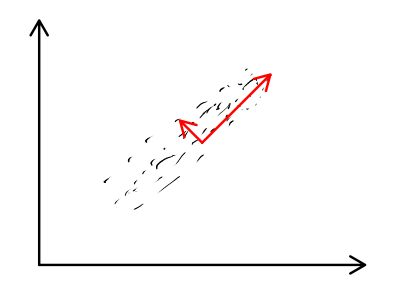
\includegraphics[width=0.25\textwidth]{Bild012}
                    \caption{PCA Beispiel}
                \end{figure}
                Dann geben die Eigenwerte $\lambda_i$ die Varianzen der $x_i$ in Richtung $v_i$ an. D.h. die $x_i$ haben in Richtung 
                $v_i$ die größte Varianz, etc.
            \end{example}

            \begin{example}\label{b4.6}
                
                Das Schwingen einer Trommel der Form $\Omega\subset \R^2$, offen, mit Frequenz $\lambda$ erfüllt
                \begin{align*}
                    \Delta u(x)&=\lambda u(x), & x\in\Omega \\ 
                    u(x)&=0, & x\in\delta\Omega 
                \end{align*}
                Mit einem ähnlichen Vorgehen wie in Kapitel 3.1 erhalten wir ein Matrixeigenwertproblem 
                \[
                    Ax=\lambda x    
                \]
                Ein Beispiel für $A$ ist Beispiel \ref*{b3.1}. $A$ ist immer spd. Alternative Diskretisierungsmethoden 
                füren auf 
                \[
                    Ax=\lambda Bx    
                \]
                mit $A,B$ spd, sehr groß und dünn besetzt.

            \end{example}

            \begin{remark}\label{b4.7}
                Sei $A\in\C^{n\times n}$.
                \begin{enumerate}
                    \item Die EW von A sind die Nullstellen de charakteristischen Polynoms
                        \[p_A(\lambda) = \det(A-\lambda I)\]
                        \[p_A\in\Pi_n\implies p_A\text{ hat } n \text{ komplexe Nullstellen}\]
                        $\implies A $ hat $n$ (möglicherweise gleiche)  Eigenwerte.
                    \item Für $A$ hermitisch $A=A^*$ sind die EW reel. Die zugehörigen EV können als ONB genutz werden. Falls $A$ zusätzlich reell ist, können die EV reell
                        und orthogonal gewählt werden.
                    \item $A\in\R^{n\times n},Ax=\lambda x$ ($\lambda\in \C$ möglich), so folgt 
                        \[A\overline{x}=\overline{Ax}=\overline{\lambda x} = \overline{\lambda}\overline{x}\]
                        $\implies (\overline{\lambda},\overline{x})$ ist auch ein EP.
                    \item Die EW zu einem Gegeben EW sind \underline{nicht} eindeutig:
                        \[Ax=\lambda x \implies Ay=\lambda y,y=\alpha x,\alpha\in\C\setminus\{0\}\]
                        \begin{align*}
                            Ax_1=\lambda x_1 \\
                            Ax_2=\lambda x_2\\
                            \implies A\alpha x_1 +\beta x_2 = \lambda(\alpha x_1 +\beta x_2)
                        \end{align*}
                    \item hnliche Matrizen, d.h. Matrizen der Form $B=CAC^{-1}$, $C$ regulär, haben die gleichen EW.
                \end{enumerate}
            \end{remark}

            \underline{\textbf{Frage:}} Was können wir sonst noch sagen? 
        
        \section{Gerschgorin-Kreise (Abschätzungen für EW)}

            Sei $(\lambda,x)$ ein EP von $A\in\C^{n\times n}$. Betrachte die $l$te Zeile von $Ax=\lambda x$:

            \begin{equation}\label{g4.3}
                \lambda x_l = \sum_{j=1}^n a_{l_j}x_j=a_{ll}x_l+\sum_{j=1,j \neq l}^n a_{l_j}x_j
            \end{equation}


            Sei $i$ so, dass $\vert x_i\vert =\max_{j=1,\dots, n}|x_j|>0$.

            Dann gilt: 
            \begin{align*}
                \left\vert \lambda -a_{ii} \right\vert \left\vert x_i \right\vert &= \left\vert (\lambda-a_{ii})x_i \right\vert\\
                &\stackrel{(\ref{g4.3})}{=}\left\vert \sum_{j=1,j\neq i} a_{ij}x_j \right\vert\\
                &\leq \sum_{j=1,j\neq i}^n \left\vert a_{ij} \right\vert \left\vert x_i \right\vert \\ 
                &\leq \vert x_i \vert \sum_{j=1,j\neq i}^n \left\vert a_{ij} \right\vert \coloneqq r_i
            \end{align*}

            \[\implies \left\vert \lambda a_{ii} \right\vert\leq \sum_{j=1,j\neq i}^n \vert a_{ij}\vert= r_i\] % TODO: Fix

            $\implies$ $\lambda$ liebt in einem Kres mit Radius $r_i$.

            \underline{\textbf{Aber:}} $x$ ist unbekannt $\implies$ $i$ ist unbekannt 

            $\implies \lambda$ liebt in der Vereinigun aller solche Kreise

            \noindent
            \xrfill[0.7ex]{1pt}Ende von Vorlesung 12 am 22.11.2022\xrfill[0.7ex]{1pt}
        
            \begin{theorem}\label{s4.7}[Satz von Gerschgorin]
                Alle Eigenwerte einer Matrix $A\in\C^{n\times n}$ liegen in 
                \[\bigcup_{i=1}^n K_i\] mit 
                \[K_i=\{z\in\C: \left\vert z-a_{ii} \right\vert \leq r_i\},r_i=\sum_{j=1,j\neq i}^n \left\vert a_{ij} \right\vert, i=1,\dots,n\]
            \end{theorem}

            \begin{proof}
                Oben.
            \end{proof}

            %Bild

            \begin{remark}\label{b4.8}
                \begin{enumerate}
                    \item Bilden $k$ Geschkorin-Kreise eine von den restlichen Kreisen disjunkte 
                    Punktmenge, so liegen in dieser Punktmenge genau $k$ EW.
                    \item Ist $A\in\R^{n\times n}$, dann haben $A$ und $A^t$ die gleichen Eigenwerte. 
                    $\implies$ EW von A liegen im Durchschnitt der jeweiligen Kreise.
                    \item 
                \end{enumerate}
            \end{remark}

        \section{Kondition des Eigenwertproblems}

            \underline{\textbf{Wiederholung:}} Die Kondition deschreibt, wie sich Änderungen in den
            Eingabedaten auf die Werte der Ausgabe auswirken. 
            \[
                \kappa_{\text{abs}}=\left\vert f'(x) \right\vert = \frac{\Delta y}{\Delta x}    
            \]

            \underline{\textbf{Frage:}} Ist das Eigenwertproblem gut- oder Schlechtkonditioniert?

            \begin{tcolorbox}[enhanced,breakable,
            title=Kondition des Problems]
            In Matrix \& Computations ist das ausführlich beschrieben. 
            \end{tcolorbox}
            

            \begin{example}\label{b4.9}
                Sei $\begin{bmatrix}
                    0 &1\\ 0&0
                \end{bmatrix}\implies $ EW sind $\lambda_{1/2}=0$.

                Sei $\tilde{A}=\begin{bmatrix}
                    0 & 1 \\ \delta & 0
                \end{bmatrix},\delta>0 \implies $ EW sind $\lambda_{1/2}=\pm\sqrt{\delta}$.

                \begin{equation*}
                    \kappa_{\text{abs}}=\frac{\left\vert 0-\pm\sqrt{\delta} \right\vert}{\left\Vert A-\tilde{A} \right\Vert_2} = \frac{\left\vert \sqrt{\delta} \right\vert}{\left\vert \delta \right\vert} \stackrel{\delta\to 0}{\to}\infty
                \end{equation*}

                Daher ist das Eigenwertproblem in diesem Fall schlechtkonditioniert.

            \end{example}

            \begin{remark}\label{b4.10}
                Allgemeiner kann man zeigen, dass (DAH Satz 5.2) die absolute Kondition eines einfachen Eigenwerts 
                $\lambda$ von $A\in\C^{n\times n}$ bzgl. $\left\Vert \cdot \right\Vert_2$ gegeben ist durch 
                \[\kappa_{\text{abs}}=\frac{\left\Vert x \right\Vert\left\Vert y \right\Vert}{\langle x,y \rangle_2} = \frac{1}{\left\vert \cos(\angle(x,y)) \right\vert}\]
                wo bei $Ax=\lambda x$ (Rechtseigenvektor) und $A^* y = \bar{\lambda} y$ (Linkseigenvektor).
                D.h. einfache Eigenwerte hermitischer Matrizen sind gutkonditioniert, da $x$ parallel zu $y$ ist. 
                
                Bei mehrfachen oder nahe zusammenliegenden EW ist die Berechnung einzelner EV-Suche schlechtkonditioniert.
                Die Berechnung einer ONB des zugehörigen Eingenpaars ist aber gutkonditioniert.
            \end{remark}
           
            \begin{remark}\label{b4.11}
                Die kanonische Idee die Eingenwerte als Nullstellen des charakteristischen Polynoms zu berechnen ist schlechtkonditioniert. Tatsächlich wird die Nullstellenberechnung in der Praxis
                als Matrixeigenwertproblem gelöst.
            \end{remark}

            \begin{tcolorbox}[enhanced,breakable,
                title=Berechnung der EW]
                    $(x-1)(x-2)\cdot \dots \cdot (x-20)$ ist ein gutes Beipsiel, warum das berechnen von Nst (hier Eigenwerten) schwer ist, weil die Koeffizienten sehr groß werden.
                    Außerdem ist das Berechnen des Polynoms, durch Berechnung der Determinante, teuer.
            \end{tcolorbox}

        \section{Vektoriteration (Potenzmethode, etc)}

            \underline{\textbf{Idee:}} Multipliziere die Matrix mit einem Vektor.

            \underline{\textbf{Iterationsfolge:}} Gegeben $A\in\C^{n\times n},x_0\in\C^n$, setze \[x_{k+1}=Ax_k\]

            \begin{theorem}\label{s4.12}
                Sei $A\in\R^{n\times n},x\in\R^n$ mit $A=A^t$ symmetrisch, mit einfachem betragsmäßig 
                größtem EW $\lambda_1$, d.h. 
                \[\vert \lambda_1\vert > \left\vert \lambda_2 \right\vert \geq \dots \geq \left\vert \lambda_n \right\vert\geq 0.\]
                Sei $x_0^tu_1\neq 0,u_1$ EV zu $\lambda_1$. Dann konvergiert 
                \begin{equation*}
                    y_k=\frac{x_k}{\left\Vert x_k \right\Vert}, x_{k+1}=Ax_k,k=0,1,\dots 
                \end{equation*}

                zu $u_1$. Die Konvergenz ist alternierend, falls $\lambda_1<0$.

                Außerdem gilt 
                \begin{equation}\label{g4.4}
                    y_k^t Ay_k\stackrel{k\to\infty}{\to}\lambda_1
                \end{equation}

            \end{theorem}

            \begin{proof}
                Sei $u_1,\dots,u_n$ eine ONB von $\R^n$ aus EV von $A$, mit $u_i$ EV von $\lambda_i$. 
                Sei

                \begin{equation}\label{g4.5}
                    x_0=\sum_{i=1}^n\alpha_i u_i
                \end{equation}
                \begin{equation*}
                    \implies x_k=A^kx_0\stackrel{\ref{g4.5}}{=}\sum_{i=1}^n\alpha_i A^k u_i = (\star)
                \end{equation*}

                \begin{align*}
                    (\star) &= \sum_{i=1}^n\alpha_i \lambda_i^k u_i\\
                    &= a_1\lambda_1^ku_1 + \sum_{i=2}^n\alpha_i \lambda_i^k u_i\\
                    &= a_1\lambda_1^k \underbrace{\left(u_1+\sum_{i=2}^n\frac{\alpha_i}{\alpha_1} \frac{\lambda_i^k}{\lambda_1^k} u_i\right)}_{=z_k\stackrel{k\to\infty}{\to} u_1}
                \end{align*}

                \begin{align*}
                    y_k&=\frac{x_k}{\left\Vert x_k \right\Vert}\\
                    &=\frac{\alpha_1\lambda_1^kz_k}{\left\Vert \alpha_1\lambda_1^kz_k \right\Vert}
                    &=\begin{cases}
                        =\pm \frac{z_k}{\left\Vert z_k \right\Vert_2}\to \pm u_1 & \lambda_1 >0 \\ 
                        =\pm(-1)^k\frac{z_k}{\left\Vert z_k \right\Vert_2}\to \pm u_1 & \lambda < 0
                    \end{cases}
                \end{align*}

                \underline{\textbf{z.z.:}} (\ref{g4.4})
                \begin{align*}
                    \left\vert y_k^tAy_k-\lambda_1 \right\vert &= \left\vert y_k^tAy_k-\lambda_1y_k^ty_k \right\vert\\ 
                    &= \left\vert \frac{x_k^t(A-\lambda_1I)x_k}{x_k^t x_k} \right\vert \\
                    &= \left\vert \frac{x_0^tA^{2k}(A-\lambda_1 I)x_0}{x_0^t A^{2k}x_0} \right\vert\\ 
                    &\stackrel{\ref{g4.5}}{=}\left\vert \frac{\sum_{i=1}^n \alpha_i^2\lambda_i^{2n}(\lambda_i-\lambda_1)}{\sum_{i=1}^n\alpha_i^2\lambda_i^{2k}} \right\vert = (\star \star)
                \end{align*}

                \begin{align*}
                    (\star\star) = \max_{i=2,\dots,n}\left\vert \lambda_i-\lambda_1 \right\vert \underbrace{\left\vert \frac{\sum_{i=2}^n\alpha_i^2\lambda_i^{2k}}{\alpha_1^2\lambda_1^{2k}} \right\vert}_{=\frac{1}{\alpha_1^2}\sum_{i=2}^n \alpha_i^2 \left(\frac{\lambda_i}{\lambda_1}\right)^{2k}} %Todo}
                \end{align*}

            \end{proof}

            \begin{remark}\label{4.13}
                \begin{enumerate}
                    \item Um Overflow/Underflow zu vermeiden, muss die Iteration angepasst werden:
                        \[y_0=\frac{x_0}{\left\Vert x_0 \right\Vert_2},y_1=Ay_k,y_k=\frac{x_k}{\left\Vert x_k \right\Vert_2}, k=0,1,\dots \]
                        Die Eigenschaften bleiben unverändert.
                    \item Der Satz \ref{s4.12} gilt aich für mehrfache EW $\lambda_1$.
                    \item In der Praxis ist $x_0^tu_1\neq 0$ wegen Rundungsfehlern nicht von Bedeutung, muss also nicht übeprüft werden.
                    \item Die Konvergenzgeschwindigkeit hängt von $\left\vert \frac{\lambda_2}{\lambda_1} \right\vert$ ab. Falls $ \vert \lambda_1 \vert \approx \vert \lambda_2 \vert $ konvergietr das Verfahren sehr langsam.    
                \end{enumerate}
            \end{remark}



            \noindent
            \xrfill[0.7ex]{1pt}Ende von Vorlesung 13 am 24.11.2022\xrfill[0.7ex]{1pt}
            

\end{document}